%%% DOCUMENT PREAMBLE %%%
\documentclass[11pt, twoside]{article}

\usepackage[english]{babel}
\usepackage{url}
\usepackage[utf8x]{inputenc}
\usepackage{amsmath}
\usepackage{graphicx}
\usepackage{subcaption}
\usepackage{parskip}
\usepackage{fancyhdr}
%\usepackage{vmargin}
\usepackage[left=38mm, right=19mm, top=20mm, bottom=20mm]{geometry}
\usepackage{nomencl}
\usepackage[breaklinks]{hyperref}
\usepackage[numbib,notlof,notlot,nottoc]{tocbibind}
\usepackage{booktabs}
\usepackage{longtable}
\usepackage{array}
\usepackage{setspace}
\usepackage{multicol}

\graphicspath{{images/}}
% Header and page number
\title{Asteroid Mining Poker}
\author{Jack Michael Sivyer}
\makeatletter
\def\cleardoublepage{\clearpage\if@twoside \ifodd\c@page\else
	\hbox{}\thispagestyle{empty}\newpage\if@twocolumn\hbox{}\newpage\fi\fi\fi}

\let\thetitle\@title
\let\theauthor\@author
\let\thedate\@date
\makeatother
\pagestyle{fancy}
\fancyhf{}
\rhead{\theauthor}
\lhead{\thetitle}
\cfoot{\thepage}
% Make arrays look nice
\renewcommand\arraystretch{1.2}
\setstretch{1.2}

\begin{document}
\large
\newgeometry{margin=1in}

% TITLE PAGE
\begin{titlepage}
\centering
% Uni logo and course code

\includegraphics[scale = 0.7]{southampton_logo.png}\\[3.7 cm]
\textsc{\Large FEEG3003 Individual Project }\\[0.5 cm]
% Big Title
\rule{\linewidth}{0.2 mm} \\[0.4 cm]
{\huge \bfseries \thetitle}\\
\rule{\linewidth}{0.2 mm} \\[1.5 cm]
Submitted by: Jack Michael Sivyer\\
Project Supervisor: Prof. Alexander Wittig\\
Date: 3rd May 2019\\
Word count: 9971
\\[6.5cm]
\textit{This report is submitted in partial fulfilment of the requirements for MEng Aeronautics and Astronautics, Faculty of Engineering and Physical Sciences, University of Southampton.}
\end{titlepage}

% DECLARATION
\cleardoublepage
\restoregeometry
\phantomsection
\addcontentsline{toc}{section}{Declaration}
\pagenumbering{roman}
{\huge\textbf{Declaration}}\\[0.7 cm]
I, Jack Michael Sivyer declare that this thesis and the work presented in it are my own and has been generated by me as the result of my own original research.
I confirm that:\\
\begin{enumerate}
	\item This work was done wholly or mainly while in candidature for a degree at this University;
	\item Where any part of this thesis has previously been submitted for any other qualification at this University or any other institution, this has been clearly stated;
	\item Where I have consulted the published work of others, this is always clearly attributed;
	\item Where I have quoted from the work of others, the source is always given. With the exception of such quotations, this thesis is entirely my own work;
	\item I have acknowledged all main sources of help;
	\item Where the thesis is based on work done by myself jointly with others, I have
	made clear exactly what was done by others and what I have contributed myself;
	\item None of this work has been published before submission.
\end{enumerate}

% ACKNOWLEDGEMENTS
\newpage
\phantomsection
\addcontentsline{toc}{section}{Acknowledgements}
{\huge\textbf{Acknowledgements}}\\[0.7cm]
With many thanks to my supervisor, Professor Alexander Wittig, who has provided much encouragement, guidance, and motivation throughout this project.

A small thanks also to my fellow students: Comerford, Freckleton, Lovelock, Peploe, and Simpson. For taking on this competitive project with a good nature and helping me to think outside the box.

% TABLE OF CONTENTS
\newpage
\phantomsection
\addcontentsline{toc}{section}{Contents}
\tableofcontents
\pagebreak
\renewcommand{\thesection}{\arabic{section}}

% LIST OF ABBEREVIATIONS
\newpage
\phantomsection
\addcontentsline{toc}{section}{List of Abbreviations}
{\huge\textbf{List of Abbreviations}}\\
\begin{description}
	\item[AI] Artificial Intelligence
	\item[CDF] Cumulative Density Function
	\item[EV] Expected value
	\item[MCTS] Monte Carlo Tree Search
	\item[PDF] Probability Density Function
	\item[NEA] Near Earth Asteroid
\end{description}

% ABSTRACT
\newpage
\vspace*{6.6cm}
\begin{abstract}
	Accurate models for real world economic applications are essential to experiment with different approaches and strategies needed to succeed in a chosen industry. This project explored incorporating game theoretical approaches to one such model based on asteroid mining: a game called \textit{Asteroid Mining Poker}. The aim was to find out what strategies succeeded with this model, whilst simultaneously researching it to find out how well it modelled the industry. The problem is approached by developing various strategies set to win specific goals relating to the game. Results showed the game partially modelled aspects of real world engineering challenges for the industry, albeit simply. It is also shown how applied game theoretical approaches can produce a consistently good strategy in the model, achieving goals beyond expectations. Concluding remarks end with recommendations for future experiments by trying different strategy types. We also make clear the changes that could be implemented to make the model more accurately represent real world situations.
	\thispagestyle{plain}
	\addcontentsline{toc}{section}{Abstract}
\end{abstract}

% MAIN REPORT
\cleardoublepage
\pagenumbering{arabic}
\normalsize

\section{Introduction} \label{Introduction}

Many aspects of the real-world economy are modelled by game theoretical approaches, this is also true for the space industry. This report focuses on a model made to apply the same approaches to a very particular part of the space industry: asteroid mining.

To experiment with the economics of a currently inactive industry (asteroid mining), accurate models need to be developed. One such model, created by professors Alexander Wittig and Ati Sharma, was made to do this: a game governed by a set of simple rules. This is achieved by allowing a few discrete events with highly variable outcomes to have big economic consequences. The game is named \textit{Asteroid Mining Poker}, in reference to both the theme and this randomness.

By performing a full theoretical analysis of \textit{Asteroid Mining Poker}, it can be determined whether this game is a good economic model. As well as this, producing strategies for the game that achieve particular goals (\textit{most money made, all-time leader in wins, recent leader in wins, and most non-bankruptcies}) are important as they can show what succeeds with the model. Furthermore, development of these strategies can highlight flaws and make improvements clear.

This project was conducted competitively involving six students in total. This report does not concern their results, but it is important to state that without their contribution, the model could not function correctly. The surnames of these students appear throughout this report. These other students are referred to as: Comerford, Freckleton, Lovelock, Peploe, and Simpson. As well as this, Evie, a control robot was used to represent an additional player who played consistently simply. Peploe's data is occasionally omitted from results, as he dropped out of the experiment towards the end.

In Section \ref{Introduction}, the problem is introduced, along with specific theory and background needed to understand it. Section \ref{Methods} covers the hypothesis and methods used to test it. Section \ref{Section3} presents the experimental results and details how did the experiment went. Finally Section \ref{Section4} presents the analysis of these results and discusses their implications.

\subsection{Background}
All relevant background information that needs to be known in order to understand the project is covered in this section. This report discusses in depth the principles of game theory. The word 'game' in this context can be defined as the following: \textit{any set of circumstances that has a result dependent on the actions of two or more decision-makers (players)} \cite{myerson2013game}.

For a certain set of strategies, the game produces a Nash equilibrium. This is a situation where every player is best off not changing their strategy \cite{nash1951non}. This is particularly common for games where players optimize for different goals such as this one. 

This report also refers to the prisoner’s dilemma. The prisoner’s dilemma is a hypothetical situation in which two players can choose either to ‘cooperate’ or ‘defect’. For both players, individually, defecting gives the greater reward. Despite this, the group benefits as a whole if both players cooperate. ‘The Dynamics of Norms’ is a book where the iterated prisoner’s dilemma is experimented with \cite{bicchieri1997dynamics}. The auction system in the game can parallel this, all players can keep the price the same (and benefit), or one player can raise the price (and benefit more). These ideas are used in the strategy development phase (Section \ref{Methods}), especially when experimenting with cooperation.

The game involves many elements of randomness. This means a pure strategy could not work. A pure strategy defines a specific move or action that a player will follow in every possible situation in the game \cite{Strategy8:online}. Developing AI to deal with randomness is discussed in Monroe’s ‘AI holds the better hand’ \cite{monroe2018ai}, which shows that games with intrinsic randomness can be ‘weakly solved’.

The game uses a first-price auction. This is an auction type where all players submit a sealed-bid and the highest bidder(s) wins. These auctions can develop an equilibrium price over many iterations (see B. Lebrun's "Existence of an equilibrium in first price auctions" \cite{lebrun1996existence}). This equilibrium principle is drawn on to develop a theoretical strategy. 

\subsection*{Asteroid Mining}
Asteroid mining is currently prohibited by the United Nations under the Outer Space Treaty \cite{OuterSpaceTreaty}. This means the model cannot be backed up by experimental data. Despite this, it can be tested against logical conclusions and known properties of asteroids. For example, asteroids can contain large amounts of material that is extremely rare on Earth, including: gold, silver, platinum, copper, indium, lead, and palladium \cite{sonter1997technical}. This shows that asteroid mining is potentially very profitable. The game incorporates this by modelling the high variability in asteroid price that would be expected from the presence -- or lack of -- these materials. This is reviewed throughout the report, it is also dedicated Section \ref{sec:FindingsAM} in context of the full properties of the game.

\subsection*{Economic Game Theory and Poker}
While game theory has been around for a long time \cite{screpanti2005outline}, Artificial intelligence (AI) using game theoretical techniques has only recently started beating humans for games such as ‘Poker’ \cite{monroe2018ai}. This is because of the intrinsic randomness in such games. Viable near-Earth asteroids can only be captured within a small-time window \cite{sonter1997technical}, the value of which cannot be perfectly known. Thus, by combining these principles, the game models a randomness similar to that seen in Poker. By developing an AI strategy that uses game theoretical approaches discussed, the model can be tested to see if it exhibits the same behaviour as real-world economic models.

\subsection{The Game}
All players were given a rules file detailing how the game worked. Over the course of the project, a few changes to the rules were discovered (see Section \ref{Section32}). This section details how the game worked with these changes taken into account.

Each game of \textit{Asteroid Mining Poker} is hosted on a private server, to which all players involved upload strategies. Players cannot see each other's strategies. Every ten minutes a game is run off the server. For each of these, two downloadable logs are produced that show what happened in game. These are referred to as the local log and the global log. For all intense and purpose, the local log contains all useful information. The primary purposes of the global log are debugging strategies and tracking player's bankrolls (necessary if a bankruptcy occurs, which renders the local log useless).

Each game works as follows: All players are assigned a \textit{bankroll} as well as a \textit{tech} value. Bankroll is what each player tries to maximize, it has an initial value of 1000. Like bankroll, tech is also accumulated by players, however, it is only used to accrue a greater bankroll. Tech is not credited to players at the end of a game and has an initial value of zero.

At the start of each round, all players lose five bankroll and are given an unknown base tech. An asteroid then appears with a stated base value and a hidden value which is not revealed. Players then bid on tech (through a first price sealed-bid auction) and decide whether they will launch for the asteroid. If nobody launches, another auction is opened, and the process repeats until a player chooses to launch. When a player does launch, all players are given another option to join the launch (given the additional information of who won the auction). The game then chooses a player or ‘Mission failure’ to mine the asteroid. It chooses this based on the amount of tech each launching player has (see Equation \ref{eq:5}). All players who chose to launch lose all their tech and five bankroll. The total value of the asteroid, plus a tech value (dependant on total tech launched) is added to the winning player’s bankroll. The game then repeats this whole process 200 more times, for a total of 201 rounds. The winner is the player ending with the highest ending bankroll. If any player's bankroll drops below zero throughout all of this, they are removed from the game. If only one player is left, the game is terminated early and the remaining player wins. Figure \ref{GameVisual} shows a visual representation of this logic process for a single round.

\begin{figure}
	\centering
	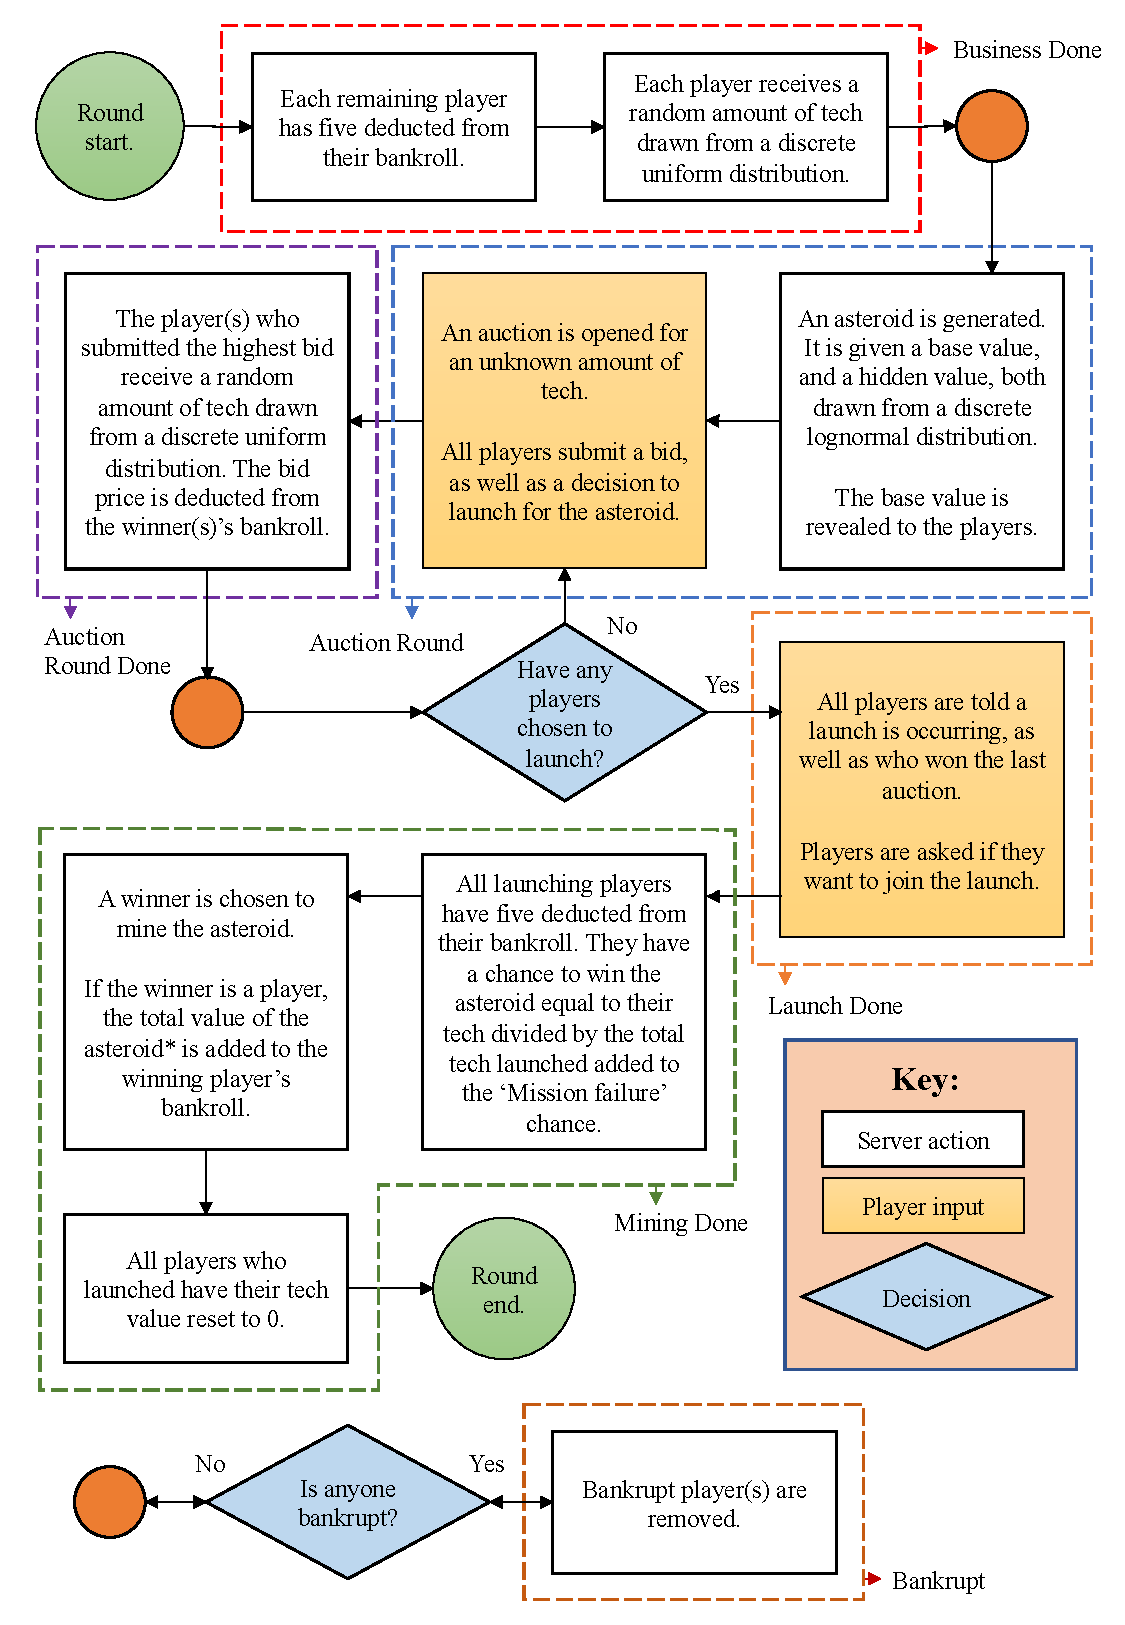
\includegraphics[width=\textwidth, height=0.9\textheight,keepaspectratio]{NewGameDesign.pdf}
	\caption{Flow diagram to give a round by round visualization of the game as seen by the server. 201 rounds occur per game.\\
		* \textit{Total value of the asteroid is equal to the sum of the base value, the hidden value, and the tech reward (a function of the total tech spent that turn by all players).}}
	\label{GameVisual}
\end{figure}

A few terms to describe some of the important game mechanics are frequently used throughout this report. These terms are outlined in Table \ref{tab:terms}.

\begin{table}[t!]
	\centering
	\caption{Common terms used to describe the game.}
	\label{tab:terms}
	\begin{tabular}{p{0.17\linewidth}>{\raggedright\arraybackslash}p{0.63\linewidth}}
		\toprule
		\textbf{Term} & \textbf{Description} \\
		\midrule
		Base reward / Base value & Given to the player as \textit{base reward} information. This value represents the guaranteed minimum a player can mine from an asteroid.\\
		Hidden reward / Hidden Value & The unknown component of an asteroid's value that is drawn from the same distribution as the base reward. \\
		Tech reward & Reward component of an asteroid that is a function of the total tech launched by players for the given turn.\\
		Unseen reward / Unseen Value & The total value of an asteroid, minus the base reward. This is equal to the sum of the hidden reward plus the tech reward.\\
		\bottomrule
	\end{tabular}
\end{table}

\subsubsection*{Defining the Type of Game}
It is important to define the type of game-theory game for \textit{Asteroid Mining Poker}. This is because different parts of game theory apply to different types of games. First of all, the game can be defined as a non-cooperative. This is a situation where players cannot form alliances which are not self-enforcing \cite{coopGame}. Non-cooperative game theory is therefore used to develop strategies, this focuses on predicting player behaviour and analysing Nash equilibria.

In zero-sum games, the sum of all players' gains and losses add to zero \cite{nash1951non}. Hence, a player can only succeed at the expense of others. Since bankroll is taken away at a rate not equal to the rate at which it is accrued by players, \textit{Asteroid Mining Poker} is not a zero-sum game. Importantly, this means that a strategy's success may allow for multiple winners and not depend on the failure of others.

\subsection*{Jerseys}

The last game for each day was recorded and saved permanently. A ‘jersey system’ which used the results of these games, tracked players progress over time. Four jerseys were awarded for different metrics, this was important for two reasons. Firstly, it added another competitive level to the game (across a longer period of time), this encouraged players to continuously update and change their strategies -- as would be expected in industry. Secondly, the jersey system provided a good benchmark for successful strategies in \textit{Asteroid Mining Poker}. All jerseys awarded are shown in Table \ref{tab:jersey}. Strategies in this project were optimized to win the green jersey.

The jersey system could not be used to measure a player's short-term success as it only updated once per day. For this reason, it was essential to develop a short-term jersey system, consolidating data across the 144 games that occurred every day.

\begin{table}[b!]
	\centering
	\caption{The jersey system: what each jersey is awarded for.}
	\label{tab:jersey}
	\begin{tabular}{p{0.22\linewidth}>{\raggedright\arraybackslash}p{0.58\linewidth}}
		\toprule
		\textbf{Jersey awarded} & \textbf{Reason given} \\
		\midrule
		Yellow & Highest number of wins in all recorded games. \\
		Green Jersey & Highest value for total money made, added across all recorded games. \\
		White & Least bankruptcies in all recorded games. \\
		Polka-dot & Highest number of wins across past seven recorded games, this was the same as the yellow jersey, but it had the seven-day limitation to allow for good strategies uploaded late to win. \\
		\bottomrule
	\end{tabular}
\end{table}

\subsection{Aims and Objectives} \label{sec:aims}
From this information and background, the aim of this project was to produce a strategy that successfully applied game theoretical approaches to consistently win the green jersey award, and thereby show what methods succeed with the model.

On top of this, a secondary aim also was to find out how well the game modelled actual asteroid mining.

From these aims, the objectives were to:
\begin{enumerate}
	\item Develop a strategy that:
	\begin{enumerate}
		\item Incorporated game theoretical approaches.
		\item Successfully and consistently won the green jersey award.
		\item Accurately applied a player model to the game.
	\end{enumerate}
	\item Develop an analysis program that could:
	\begin{enumerate}
		\item Determine how the game works by discovering the unknowns.
		\item Analyse outputted logs in order to visualize and improve the strategy.
		\item Analyse multiple logs and find averages in place of a short-term jersey system.
	\end{enumerate}
\end{enumerate}

\newpage

\section{Theory / Methods} \label{Methods}

Reliable methods concerning data collection and analysis were essential to the success of this project. Because of this, a python program was developed that could easily interface with the game server. This program was also used to make all of the analysis tools required (see Appendix A). From this point onwards, this is simply referred to as \textit{the program}.

\subsection{Data Collection} \label{sec:methods2}
To determine correctly how the game works, a lot of data was needed to minimize error. In order to tackle this, one function of \textit{the program} retrieves unique data from the game server as frequently as possible.

A game ran every ten minutes and had a set number of rounds (For the majority of this report the round limit was 201). Hence, the maximum rate at which data could be collected (assuming no early winners) was 28,994 general data points per day, and 144 round specific data points per day. General data, being a term to describe data not dependent on the round number, for example: data for the base reward distribution. Turn specific data on the other hand, is dependant on the round number, such as the mission failure probability per round. Because of this, turn specific distributions, required much greater amounts of data to be analysed. This can be seen as a greater error in Figures plotting results for these data sets.

For \textit{the program} to handle such large amounts of data, a function was created to put all the important data from each local log into a json file at download. To find out what constitutes important data, all necessary data items can be categorized. Table \ref{tab:data} shows each unknown in the game, along with the data needed to determine it. By constructing a simple table such as this, the data needed from each log is made clear.

\subsection{Theory Behind Strategy} \label{Section22}
Since the scores for this project were cumulative (counting from the 10th October 2018), it was necessary to quickly upload a basic strategy to generate money. To achieve this, a basic strategy was created that simply bided four and launched if it had a tech value above 20 (see Appendix B). This was done to achieve a quick lead on the jersey awards before a more complex strategy was implemented.

\begin{table}
	\centering
	\caption{Data required to determine the unknown aspects of the game.}
	\label{tab:data}
	\begin{tabular}{p{0.4\linewidth}>{\raggedright\arraybackslash}p{0.4\linewidth}}
		\toprule
		\textbf{Unknown Mechanism} & \textbf{Data required} \\
		\midrule
		Base reward distribution. & Base reward values. \\
		Tech reward function. & Unseen rewards for different tech launched values. \\
		Base tech given distribution. & Base tech given values. \\
		Auction tech won distribution. & Auction tech won values. \\
		Mission failure chance per round. & Number of times mission failure occurs per round for different amounts of tech launched. \\
		\bottomrule
	\end{tabular}
\end{table}

For this type of game, there are a few things that are logically beneficial to be hard coded into the strategy. For example, it is almost always a good thing to launch on the last round. This is because stored tech is worth nothing but what it can gain through providing a higher chance to mine asteroids. There is a cost of five to launching, so unless the expected value of the asteroid is less than five (which is rare), launching on the last round is always a good play. This is why, for the iterated prisoner’s dilemma experiment  \cite{bicchieri1997dynamics}, an unknown number of rounds was used to stop this rule being exploited.

The next two things concern bankruptcy avoidance. First of all, a strategy must always launch if the bankroll falls below five. Since five bankroll is taken at the start of each turn, choosing not to launch will always end in a bankruptcy. Hence, a strategy must always launch if the bankroll dips below five if it is to have any chance at staying in the game.

Secondly, a strategy must never bid an amount equivalent, or more than its bankroll. Even if an asteroid's pay-off is very high, systems must be in place to prevent a strategy from bankrupting itself.

For each round there are three decisions a strategy consolidates: bid amount, the initial launch decision, and the join launch decision (see Figure \ref{GameVisual}). Of these, it can be logically deduced the join launch decision is never useful. To understand why, two scenarios are considered:

Firstly, for strategies which have chosen to launch in the auction phase, the join launch decision can change nothing and is obsolete.

Secondly, considering strategies which have chosen not to launch in the auction phase, significant new data must be available to change this decision. At the join launch stage two new bits of information are made known: the winners of the last auction, and the fact that at least one other player is launching. This information can only be positive if the winner of the last auction is (or includes) the player in question. However, this is offset by the huge decrease in expected value from the knowledge at least one other player is launching. Without this information, there was a chance the player did not have to compete. This means the final expected value increase cannot be positive. Ultimately, this means that the player modelling done in the auction stage consolidates all useful sources of data and thus, the join launch decision phase is useless. This reduces the complexity of strategy development significantly.

\subsubsection*{Creating a Player Model}
A player model is a computational model which can accurately predict a player's actions. This is done by recording characteristics manifest in behavioural patterns, which are then used to make predictions of future actions \cite{yannakakis2013player}. A good model also keeps track of a player's statistics and makes estimates as to their available resources.

A good player model is a key component to winning non-cooperative games as it can be used to avoid competition and gain easy wins \cite{nash1951non}. Because of this, a heuristic player model was developed. A player model can be programmed to record and make predictions for behaviour exhibited by a player. Table \ref{tab:playerModel} shows all of the common behavioural patterns observed, as well as the data required to accurately model a player exhibiting such patterns. These observations were aided through use of the data visualization tools in \textit{the program}.

\begin{table}[b!]
	\centering
	\caption{Simple behaviours included in player model development.}
	\label{tab:playerModel}
	\begin{tabular}{p{0.3\linewidth}>{\raggedright\arraybackslash}p{0.5\linewidth}}
		\toprule
		\textbf{Observed behaviour} & \textbf{Mitigation required} \\
		\midrule
		Player not launching for first N turns. & Record when a player's strategy begins. Assume no launches until then. \\
		Player not launching for first N turns after previous launch. & Learn the minimum number of turns in between launches. Assume no launches in this gap. \\
		Player always launches within N turns of previous launch. & Record the maximum number of turns between two launches. Assume a launch if this gap is exceeded. \\
		Player always launches when their estimated tech value is above N. & Estimate a player's tech value and record its maximum value. Assume a launch is a player's estimated tech value exceeds this. \\
		Player always launches on certain rounds. & Record the rounds for which a player does not launch. Assume a launch on the rounds which are not recorded. \\
		Player will always launch above a given asteroid base value. & Record the maximum base value for which a player does not launch. Assume a launch for all asteroids above this value. \\
		Player never launches for asteroids with too low a base value. & Record minimum value for which a player launches for an asteroid. Assume no launches for all asteroids below this value. \\
		\bottomrule
	\end{tabular}
\end{table}


For strategies that did not exhibit any of the simple behaviours listed in Table \ref{tab:playerModel}, the player model based it's launch prediction on the average base value for which it was more common for a player to launch. For example, if a player launched more often than they did not for a base value of six -- but not for a base value of five -- then the player model assumed a launch for all base values above five. 

Combined with the simple observations in Table \ref{tab:playerModel}, the player model kept track of each player's bankroll and tech. Fortunately each player's bankroll was made publicly available at each stage of the game, so this did not need to be modelled. Calculating each player's tech was critically important as it was needed to determine the chance a launch succeeded. The player model did this by saving each player's most likely current tech. This is 100\% accurate for certain points in the game: the beginning of each game, and after a player has launched. After both of these events, a player's tech is known to be equal to zero. As player's accumulated tech, the player model estimated each player's tech by using averages. For both auctions won and tech granted at the beginning of each round, the player model just added the average value given from these distributions to a player's estimated tech. This meant that the player model became less accurate as players accumulated large amounts of tech.

\subsubsection*{The Ideal Strategy}
A good strategy should take into consideration all available data effecting its performance. Therefore, unknown mechanisms in Table \ref{tab:data} should be incorporated into its logic process and results from the player model must be used.

Once the unknown distributions are discovered, the probabilities of all future asteroid rewards can be calculated. This reduces all unknowns to perfect knowledge of just a few variables: the actual asteroid values, what other players will do, and how much tech players bid in auctions.

One way to use all this data would be to perform a Monte Carlo Tree Search (MCTS) for every launch decision. A MCTS is a search method that combines the precision of the tree search with the generality of random sampling \cite{browne2012survey}. A MCTS works by assuming a 100\% correct player model, it then runs a number of simulations of the game for all future rounds. An equal number of simulations is run for both options: a launch, and no launch. Because the simulation draws from random distributions, both paths will lead to many different outcomes. A MCTS chooses whether to launch by averaging all end results for both options. The option with the highest average is chosen to be the action committed. Figure \ref{MCTSPic} shows a diagrammatic example of this process.

\begin{figure}[t!]
	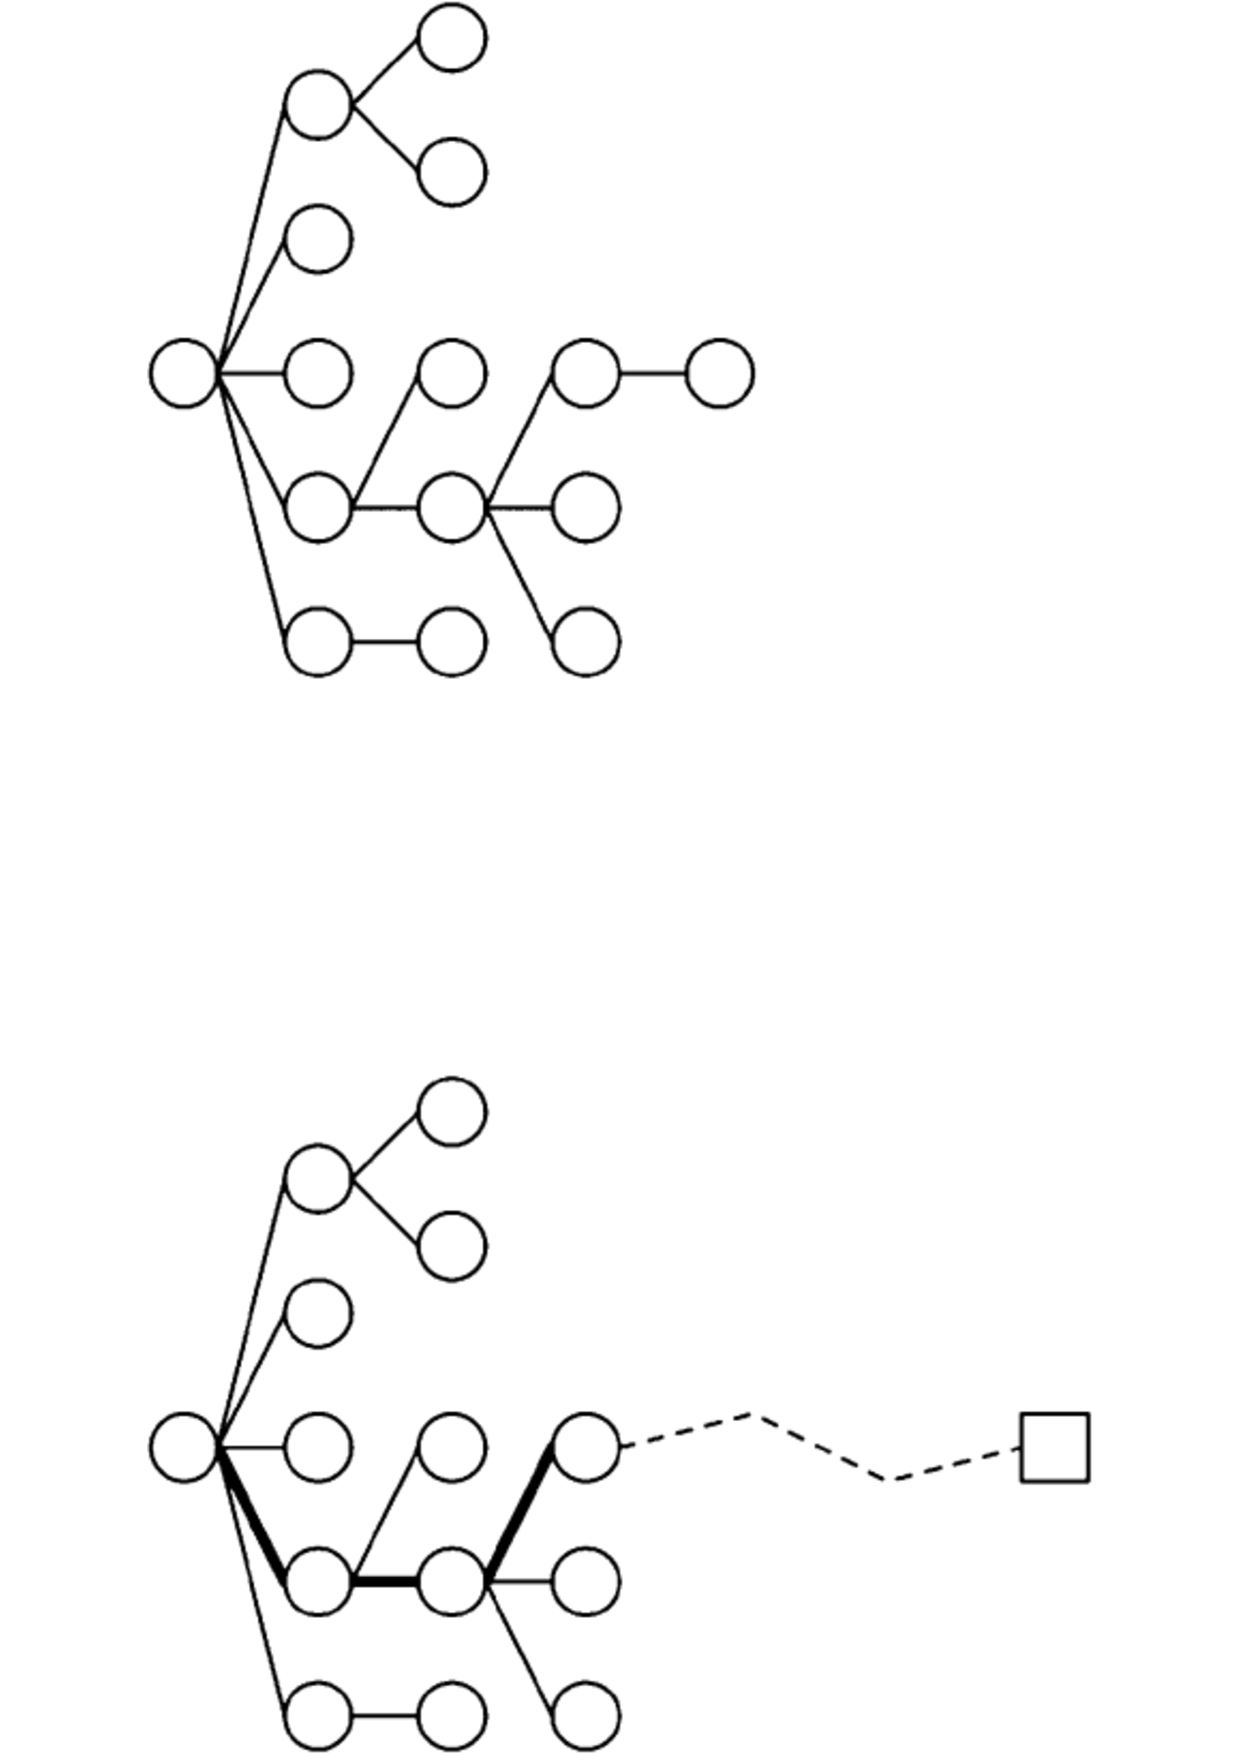
\includegraphics[height=\textwidth,keepaspectratio,angle=-90]{MCTS.pdf}
	\caption{A Monte Carlo Tree Search \cite{baier2010power}.}
	\label{MCTSPic}
\end{figure}

\subsubsection*{Choosing What to Optimize}
To improve a strategy, it has to be tested against a set standard. Only then, can the strategy be modified and adjusted to make it better. It is important to pick the right standard for this, as different metrics may have unforeseen consequences. Two options are considered:

\begin{enumerate}
	\item Maximizing pure bankroll.
	\item Maximizing faction of bankroll above next player / below winning player.
\end{enumerate}

Considering option one, maximizing bankroll has the benefit of producing a consistent strategy. This is because it ignores other players performance and optimizes for a high score, making end game bankrolls of under zero unlikely. Despite this, optimizing bankroll alone is problematic. Being not a zero-sum game, a high bankroll does not necessarily guarantee a strategy is doing well in the environment. For example, a strategy may consistently achieve an end bankroll of over 1000, however if the average ending bankroll is over 2000, this would be a bad score. To achieve the greatest money made (the green jersey), the final strategy must use another metric.

Considering option two, maximizing the bankroll fraction is beneficial because, ultimately, making the most money is measured against the success of other players. Thus, maximising the gap between a player's total score and the next player is very important. Optimizing for the bankroll fraction increases this gap. Despite this, optimizing for bankroll fraction may produce a strategy that plays with higher risk. This is because it does not take into consideration its own ending bankroll. This means that although the gap between players bankrolls are increased, more bankruptcies are to be expected.

Option two must be chosen to develop a strategy. This is because the objective is to produce a strategy that maximizes total bankroll, which is measured against other players. Therefore, increasing the mentioned gap is more important than the occasional bankruptcy.

\subsection{Development of Strategy} \label{SectionDEVSTRAT}

From first principles and by combining all of the logic discussed so far, this section shows how the final strategy was developed. This is done by detailing the logic process for each round, given the asteroid base value. Some results concerning the game have been included in this development phase.

Unfortunately, a few systems in the game were discovered that prevented the use of a MCTS. The game has a calculation timeout of just a few seconds, which is too short to perform a full MCTS. Thus, the ideal strategy had to be modified to perform a simpler calculation and yet retain many of the same principles discussed. Therefore, a simplified tree search is used: rather than running simulations until the end of the game, the strategy was modified to consider just the next round.

The disadvantage of this new strategy is that it may not make the best decision for the long term. However, considering just the next round significantly sped up calculations and allowed it to respond to other players' actions. Rather than run repeated simulations up to the end game, the new strategy asked just one question each round: is it better to launch now or later? Its operation is detailed below.

Firstly, the total tech being launched is estimated, this is done by using the player model to get an estimation of the total tech launched by others. Five is also added onto this value as at least one player always wins the auction. There is an assumption made here that only one player wins the auction, which could be improved by updating the player model to guess each player's bid amount.

\begin{equation}
	\label{eq:techReward}
	\text{tech}_{\text{total}} = \text{tech}_{\text{self}} + \text{tech}_{\text{others}} + 5
\end{equation}

Finding the total tech allows the total reward of the asteroid to be estimated. This is simply equal to the base reward plus the hidden reward and the tech reward. The only unknown of these is the hidden reward, which is assumed to be its average value of 11.05. Equation \ref{eq:techReward} comes from the analysis in Section \ref{sec:analysis1}.

\begin{equation}
	\text{reward}_{\text{tech}} = 1.207 * \sqrt{\text{tech}_{\text{total}}} - 0.413
	\label{eq:reward}
\end{equation}
\begin{equation}
	\text{reward}_{\text{total}} = \text{reward}_{\text{base}} + 11.05 + \text{reward}_{\text{tech}} - 5 \nonumber 
\end{equation}

The expected value can then be calculated. The expected value is equal to the total asteroid reward, times the probability that it is won. The probability the asteroid is won is given by the game rules: equal to tech launched divided by total tech launched added to mission failure probability. The expected value of the asteroid is also calculated for the case where the auction is won. Once again, only one player is assumed to win the auction.

\begin{equation}
	EV_{\text{auction\_lost}} = \text{reward}_{total} \times \dfrac{tech_{self}}{tech_{total}+F}
	\label{eq:EV1}
\end{equation}\\
\begin{equation}
	EV_{\text{auction\_won}} = reward_{total} \times \dfrac{tech_{self} + 5}{tech_{total}+F} \nonumber
\end{equation}

Ultimately a good strategy buys tech when it is cheap and uses it in optimal situations. This does not retract from the fact that the expected value increase on an asteroid may be great enough to justify paying a large amount of bankroll for a high return. Hence, the maximum bid can be set equal to the difference between the two expected values (Equation \ref{eq:bid}). This value is only a maximum: it would be foolish to bid this value all the time as it would act to mitigate 100\% of the extra bankroll gained. It does however, set a maximum bid.

\begin{equation}
	\text{Bid}_{\text{max}}=EV_{\text{auction\_won}} - EV_{\text{auction\_lost}}
	\label{eq:bid}
\end{equation}

A Nash equilibrium is expected to develop for non-cooperative games \cite{nash1951non}. Because of this, the strategy records the highest value other players have bid in the past three auctions. The strategy then bids one above this amount, if this is below the maximum bid. By doing this, the strategy buys tech at the lowest price required to outbid others, while never buying tech that does not return a higher probability that it would cost.

The strategy then runs through a series of logic to decide whether to launch or not. It does this by finding the probability a greater reward will be available next turn (accounting for the lost revenue from waiting). For this calculation, tech value is ignored because it has a small effect. This is another assumption that could be improved in future strategies. The logic for the launch decision is detailed below.

Firstly, the worst-case scenario is considered: given all players run perfect strategies, the asteroid rewards should be split equally. This means that a good strategy should launch for returns of at least (or equal to) the average reward divided by the number of players. Equation \ref{eq:bar} shows how this 'bar' (B) is calculated, based on player number N. Five is added onto the end of this as an assumption that only one player wins the auction each round.

\begin{equation}
	\label{eq:bar}
	B= \dfrac{22.1}{N} + \text{reward}_{\text{tech}}(\text{tech}_\text{total}=5 \times N + 5)
\end{equation}

To find the chance that the next asteroid will give a higher value the probability density function (PDF) of two log normal distributions must be calculated. The PDF of a log normal distribution is given by Equation \ref{eq:lognormal}, \cite{kotz2004continuous}.

\begin{equation}
	f_{X}(x)=\frac{1}{x}\cdot\frac{1}{\sigma\sqrt{2\pi}}\cdot \text{exp}{\left(-\dfrac{(\text{ln}(x)-\mu)^2}{2\sigma^{2}}\right) }
	\label{eq:lognormal}
\end{equation}

The cumulative function of the square of Equation \ref{eq:lognormal} is needed to find the chance the next asteroid will have a higher value. To determine this, let $Y = X^2$, where the PDF of X is $\frac{d}{dx}P(X<x)$.

\begin{align}
	P(Y < x) & = P(X^2 < X)\nonumber \\
	& = P(−\sqrt{x}<X<\sqrt{x})\nonumber \\
	& = P(0 < X < \sqrt{x}) + P(0 < -X < \sqrt{x}) \label{eq:15}
\end{align}

\vspace{0.2cm}Then, by taking the derivative of Equation \ref{eq:15}, the PDF of $Y$ can be determined \cite{813462}.

\begin{equation}
	f_{Y}(x) = \frac{1}{2\sqrt{x}}f_{X}(\sqrt{x})+f_{-X}(\sqrt{x}) \nonumber 
\end{equation}

By integrating this from zero to estimated reward for the round plus five, the chance the next asteroid has a higher value than the current reward plus five can be found (shown as $\alpha$). The five is added here to make up for the lost revenue from waiting.

\begin{equation}
	P(\text{next asteroid has higher value}) = \alpha = 1 - \int_{0}^{5+\text{reward}_{\text{total}}} f_{Y}(x) dx \nonumber 
\end{equation}

The expected value for the asteroid next turn can then be calculated as simply the reward plus five, times by the chance that it occurs.

\begin{equation}
	EV_{\text{next turn's asteroid}} = \alpha \times (\text{reward}_{\text{total}} + 5)
	\label{eq:EV2}
\end{equation}

The advanced strategy then decides to launch based on either of the following conditions:
\begin{itemize}
	\item If the turn is equal to the turn limit AND the expected value (Equation \ref{eq:EV1}) is greater than five.
	\item If the reward (Equation \ref{eq:reward}) is greater than the bar (Equation \ref{eq:bar}) AND if the next turns expected value (Equation \ref{eq:EV2}) is lower than the current turns expected value (Equation \ref{eq:EV1}).
\end{itemize}

Only one of the the conditions has to be true for a launch. If neither of these conditions are met, the strategy does not launch.

\subsection{Analysis Code Theory}
In order to spot the failures in a strategy, potential flaws and improvements; a robust data visualization method was developed. This analysis was automated by a function in \textit{the program} and produced a series of graphs for any given game log (To see the data visualizations added to the analysis and why, see Appendix C).

\newpage

\section{Analysis} \label{Section3}

\subsection{Using Data to Understand the Game} \label{sec:analysis1}

The rules of the game do not explain what distributions are used. This section concerns how these distributions were found. The unknowns in question are as follows: the base reward distribution, the tech reward function, the base tech given distribution, the auction tech won distribution, and finally, the mission failure chance per round function.

 For each of these unknown distributions, a function was added to \textit{the program} in order to find out what they were. This was done by recoding all instances of data for which these functions were involved (see Table \ref{tab:data}). The next part of this report is concerned with the results of these functions.

\subsubsection*{Finding the Asteroid Base Value Distribution}
At the beginning of each round, the base value of a new asteroid was revealed. The probability distribution from which these were drawn is plotted in Figure \ref{BaseDistribution}. Equation \ref{eq:1} shows how each data point was calculated.

\begin{equation}
\label{eq:1}
P(\text{X}) = \dfrac{\text{Observations of X}}{\text{Total number of observations}}
\end{equation}

\begin{figure}[h!]
	\centering
	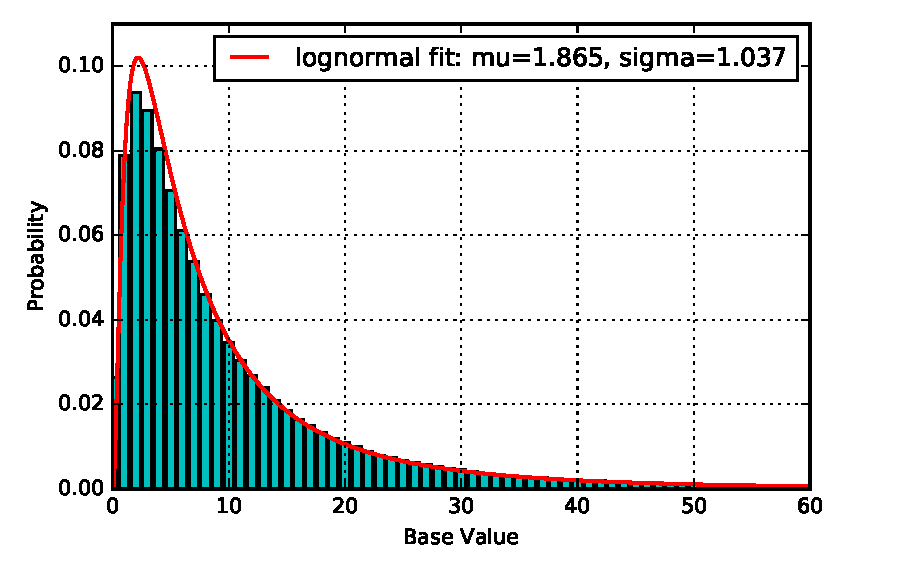
\includegraphics[width=\textwidth,keepaspectratio]{base_distribution.pdf}
	\caption{Probability distribution for the base values of asteroids. Data has a mean of 11.05 and a variance of 235.49. Data observations used in this plot: 555,917. Standard error: 0.0206.}
	\label{BaseDistribution}
\end{figure}

Due to the discrete nature of this distribution, along with an abundance of data, a bar chart was plotted for all values recorded (this is equivalent to a histogram with bin size equal to the data step). Hence, every bin in the population has been sampled equally, meaning the error is constant. The same principle is also applied to both the tech distributions and the hidden distribution.

By inspection, Figure \ref{BaseDistribution} can be seen to be a log normal distribution. By finding the mean and variance of the plot (represented by m and v respectively), values for the log normal $\mu$ and $\sigma$ are calculated with Equations \ref{eq:mu}, and \ref{eq:sigma}, \cite{forbes2011statistical}.

\begin{multicols}{2}
	\begin{equation}
		\label{eq:mu}
		\mu = log\left(\frac{m}{\left(1+\frac{v}{m^2}\right)^{0.5}}\right)
	\end{equation} \break
	\begin{equation}
		\label{eq:sigma}
		\sigma = {log\left(1+\dfrac{v}{m^2}\right)}^{0.5}
	\end{equation}
\end{multicols}

Using these values with the log normal PDF, a fitted log normal curve was added to Figure \ref{BaseDistribution}. This has been verified by the game developer to be the correct distribution.

\subsubsection*{Finding the Tech Given Distributions}

\begin{figure}[b!]
	\centering
	\begin{subfigure}[b]{0.49\textwidth}
		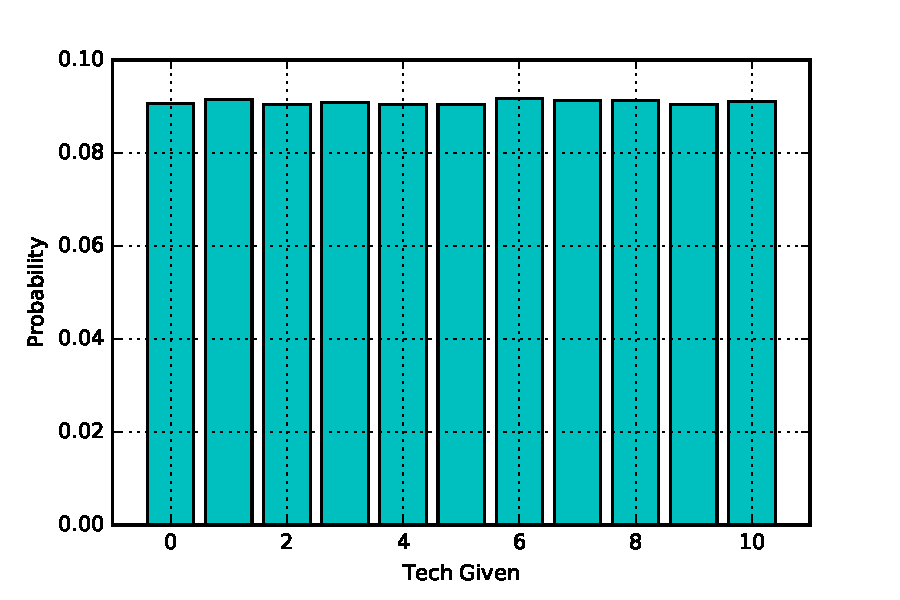
\includegraphics[width=\textwidth]{base_tech.pdf}
		\caption{Base tech distribution.}
	\end{subfigure}
	\begin{subfigure}[b]{0.49\textwidth}
		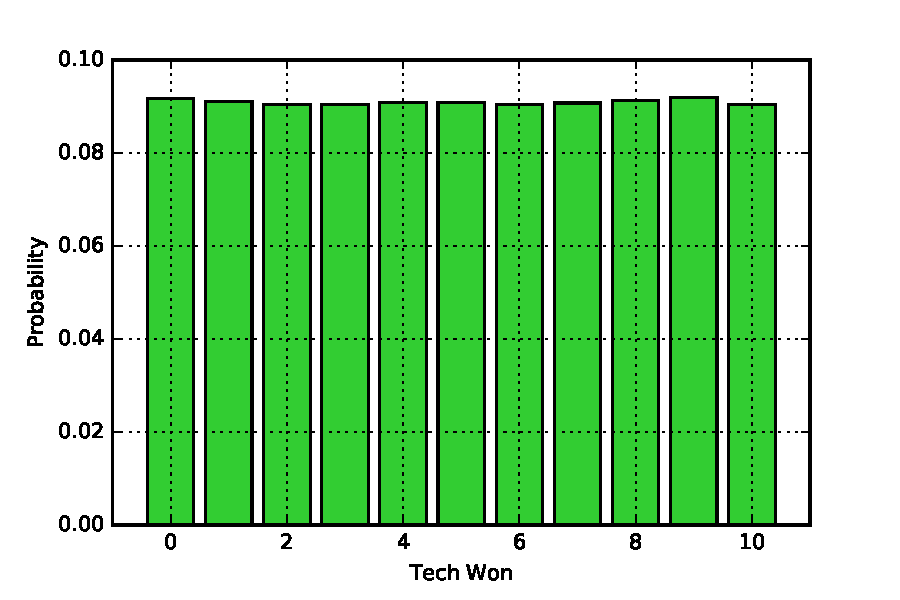
\includegraphics[width=\textwidth]{auction_tech.pdf}
		\caption{Auction tech distribution.}
	\end{subfigure}
	\caption{The PDFs showing tech awarded at different parts of the game.}
	\label{Base&TechDistributions}
\end{figure}

Similarly to the base distribution, the PDFs for the tech distributions were plotted using equation \ref{eq:1}. Data for these was collected by recording the amount of tech received for all events where tech was given. Unlike base tech data (which could be taken at the start of every round), auction tech data could only be recorded for instances the strategy being played won auctions. This means the base tech distribution has a standard error 37\% lower than that of the auction tech distribution (measured at 0.00424 to 0.00668). Fortunately, both of these values are very low, increasing confidence in the results. 

Figure \ref{Base&TechDistributions} shows that both tech distributions are the same. By inspection, these are observed to be discrete uniform distributions with a range from 0 to 10. This means that the average tech received by each player at the start of each round, and after winning an auction, is five. These distributions have been verified by the game developer to be correct.

\subsubsection*{Finding the Tech Reward Function}
The unseen value of asteroids (calculated by taking the total reward of an asteroid minus its base reward) is made up of a fixed probability distribution summed with the tech reward function (a function of tech played). Because of this, the tech reward function can be revealed by plotting the average unseen reward against tech played, and then subtracting the average value of the fixed probability distribution. This hidden distribution is stated by the game rules to be the same as the base distribution (Figure \ref{BaseDistribution}), so this average value is equivalent to 11.05.

\begin{figure}[b!]
	\centering
	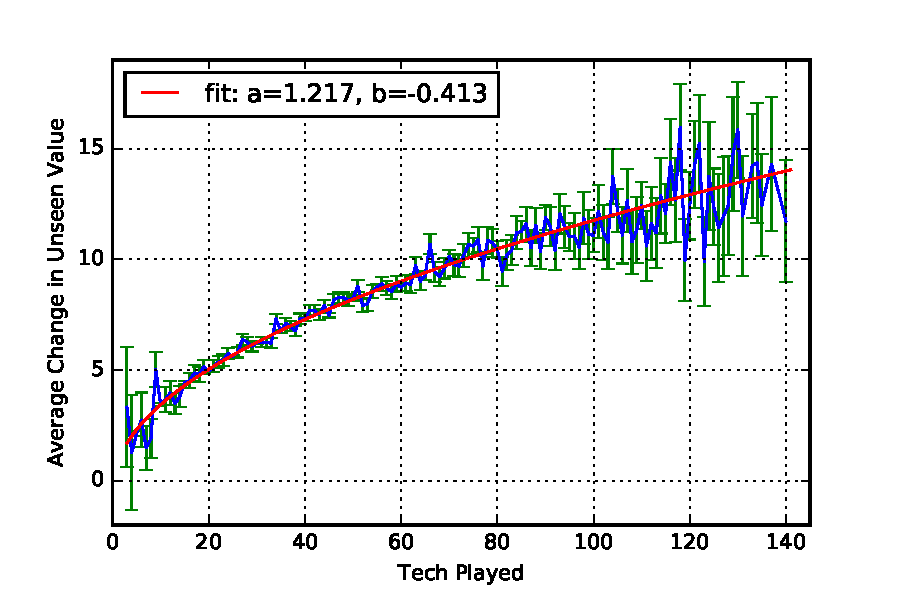
\includegraphics[width=\textwidth,keepaspectratio]{tech_function.pdf}
	\caption{Variation of average change in asteroid unseen value with total tech launched that turn. Data is plotted in blue. Error bars are shown in green. Data has been fitted with the function: $a*\sqrt{x}+b$ (red line).}
	\label{TechFunction}
\end{figure}

To use this method, the total tech launched (T) is estimated by tracking each player's tech with the player model (discussed in Section \ref{Introduction}). Because of this, the data can be expected to a greater error for increasing tech values, as player's tech values were estimated using averages. Equation \ref{eq:4} can then be used to determine the average tech reward as a function of tech played, plotted in Figure \ref{TechFunction}.

\begin{equation}
\text{F(T)}=\dfrac{\text{Average asteroid unseen value for launch tech T}}{\text{Total observations for launch tech T}} - \text{Average hidden value}
\label{eq:4}
\end{equation}

 By inspecting Figure \ref{TechFunction}, it can be seen that the tech reward is some function of the square root of total tech launched (T). An optimizer was used to fit the data, giving the tech function as $1.217 * \sqrt{T} - 0.413$. The game developer has confirmed that the tech function is indeed some function of the square root of total tech launched. The data shows high error values for the extremes of tech played. This was expected, not only for the reasons already discussed, but simply because occurrences of extreme tech values played were infrequent, so data was scarce.

\subsubsection*{Verifying the Asteroid Value Hidden Distribution}
The rules state the base and hidden distributions are the same, therefore finding the hidden distribution can be used to verify results.

\begin{figure}[b!]
	\centering
	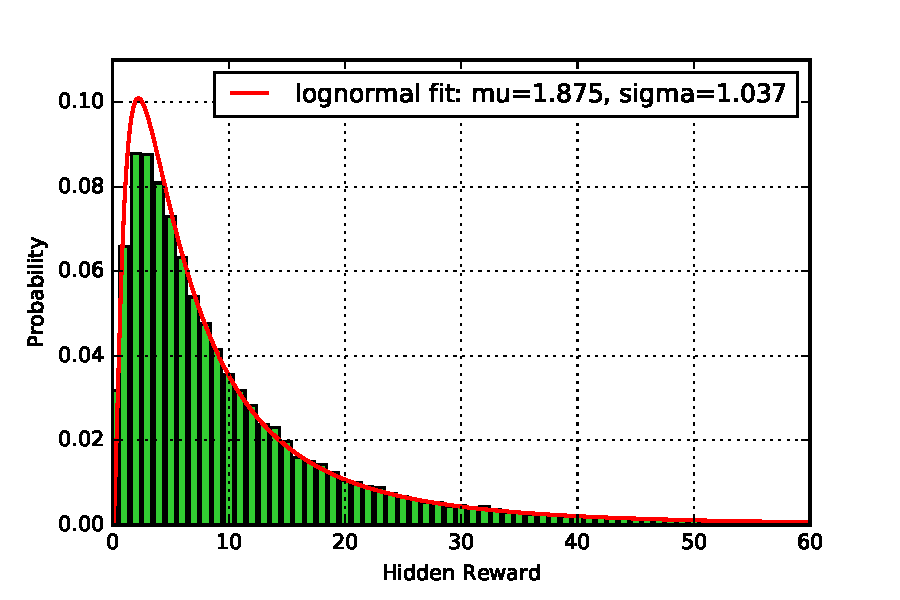
\includegraphics{hidden_distribution.pdf}
	\caption{Graph showing the normalized unseen value of asteroids for 20 tech launched with a log normal fit. All x-axis values have been shifted down by five to correct for the tech function reward.}
	\label{HiddenDist}
\end{figure}

Since the unseen reward from asteroids consisted of the tech function and a value from the hidden distribution, the hidden distribution can be plotted by looking at data for which the tech function was constant. The launch tech chosen was 20 because it was the most often recorded (59,751 occurrences), reducing error. It can be expected that the graph will resemble the base reward distribution (Figure \ref{BaseDistribution}), if each value is shifted down by the tech reward. By using the equation for the tech reward discussed, this value comes out to be five. Zero would have been a good choice in theory, however, this occurred too rarely to collect any significant data. 

Figure \ref{HiddenDist} shows the average hidden value of asteroids for just a launch tech of 20, shifted to the left by five to make up for the additional tech reward. As expected, this produces a very similar graph to the base distribution (Figure \ref{BaseDistribution}) with $\mu$ within 10\%, and the same $\sigma$. Small differences were expected due to estimates in other player's tech values. This verifies results so far.

\subsubsection*{Finding Mission Failure Tech}
Understanding the failure rate is integral to producing a good strategy that avoids it. Mission failure is modelled as a player who launches every turn, they submit a tech value like every other player (although this may be a float, unlike players). Equation \ref{eq:5} shows how the mission failure tech (F) is modelled and effects the player win rate.

\begin{figure}[b!]
	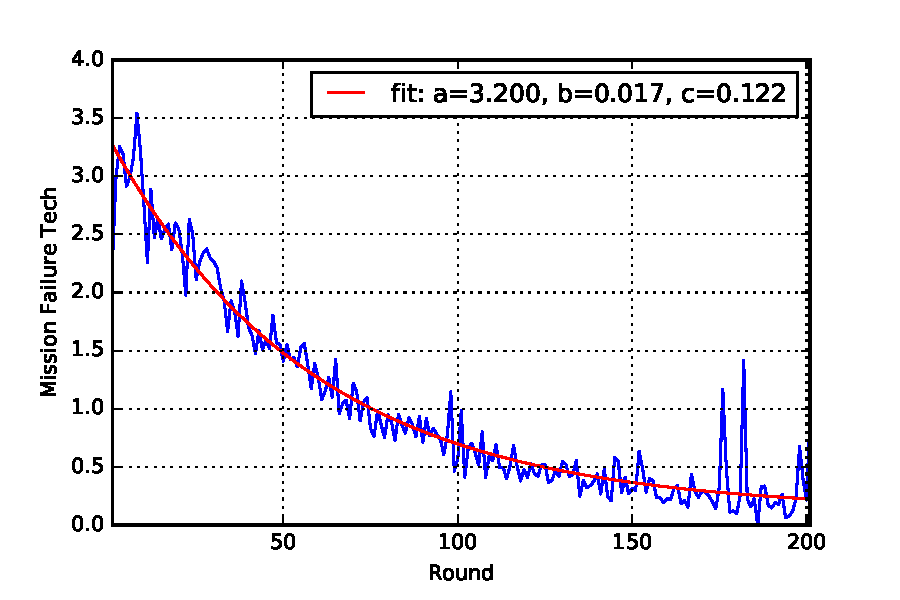
\includegraphics{mission_failure_tech.pdf}
	\caption{Variation of mission failure tech submission per round. Data has been fitted with the function: $ae^{-xb} + c$ (plotted as a red line).}
	\label{MissionFailure}
\end{figure}

\begin{equation}
	P(\text{player wins}) = \dfrac{\text{tech launched}}{\text{total tech launched} + F}
	\label{eq:5}
\end{equation}

The mission failure tech is given to be some function of the round number. Hence, by taking data for just one round, and for just one set of tech launched by all players, the failure tech can be calculated. This is done by rearranging Equation \ref{eq:5} to give Equation \ref{eq:6}.

\begin{equation}
	F = \text{Tech launched} \times \dfrac{\text{Failures observed}}{\text{Total sets observed}}
	\label{eq:6}
\end{equation}

Different sets of tech were used to get multiple results. Figure \ref{MissionFailure}, shows the weighted average of these sets, for all rounds up to 201. This produces a graph showing some form of exponential decay. An optimizer was used to fit the data, giving the mission failure submission per round as $3.2e^{-0.017x} + 0.122$. The game developer has confirmed the mission failure submission is indeed an exponential decay which is a function of round number.

\subsection{Features Discovered Through Analysis} \label{Section32}

\begin{figure}[b!]
	\centering
	\begin{subfigure}[b]{0.49\textwidth}
		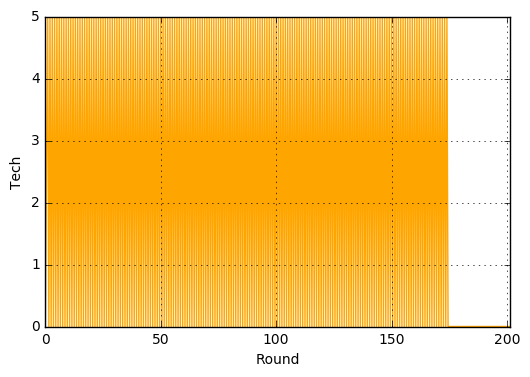
\includegraphics[width=\textwidth]{normgame_t7.png}
		\caption{Lovelock's tech variation per round.}
	\end{subfigure}
	\begin{subfigure}[b]{0.49\textwidth}
		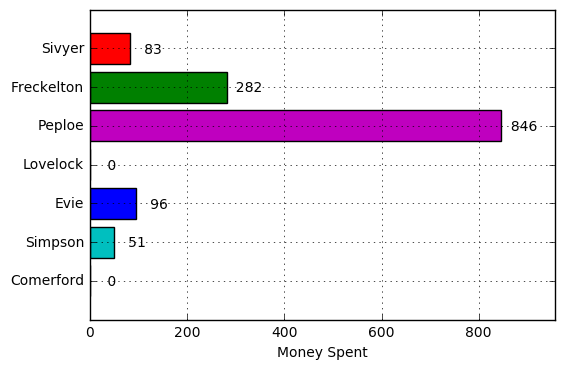
\includegraphics[width=\textwidth]{normgame_aspent.png}
		\caption{Bankroll spent on auctions per player.}
	\end{subfigure}
	\begin{subfigure}[b]{0.39\textwidth}
		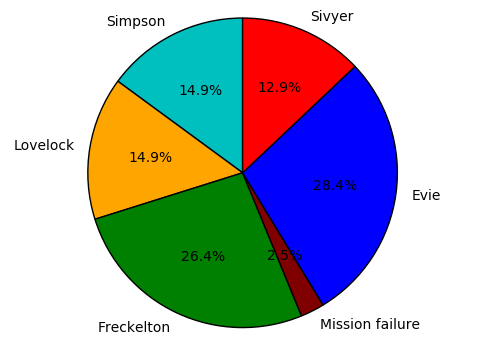
\includegraphics[width=\textwidth]{normgame_amined.png}
		\caption{Fraction of asteroids mined per player.}
	\end{subfigure}
	\begin{subfigure}[b]{0.59\textwidth}
		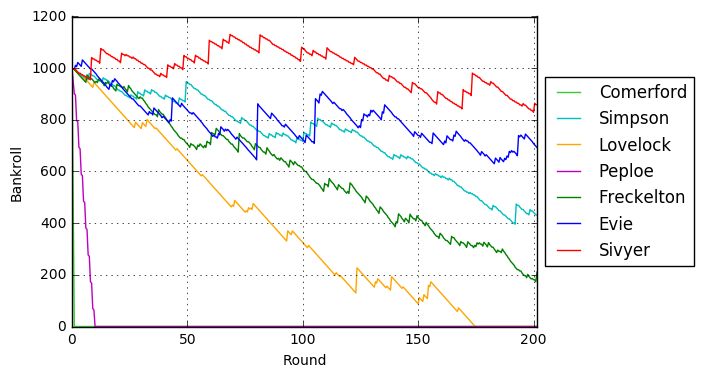
\includegraphics[width=\textwidth]{normgame_bank.png}
		\caption{Bankroll variation per round per player.}
	\end{subfigure}
	\caption{Analysis for a single game on 19$^{\text{th}}$ April 2019. This figure contains several of the data visualizations made for just one game.}
	\label{Analysis1}
\end{figure}

To spot errors in the strategies, along with areas to improve, an analysis tool was developed to review a chosen log. This tool was also useful for verifying game rules. Over the course of the project, two changes to the rules were discovered using these techniques. These changes, and how they were discovered are briefly discussed in this section.

The output of just one analysis is shown in Figure \ref{Analysis1}. The first change to the rules was discovered by observing the rate of decay in players' bankrolls. Players who did not launch or bid in auctions, can be seen to lose bankroll at a rate of five per turn. In the original rules, this was said to decay at a rate of ten per turn.

The second change can also be deduced from Figure \ref{Analysis1}. Observation of player Lovelock's tech shows that the strategy launched every turn. Lovelock also spent zero bankroll in auctions. Despite this, the player won a few asteroids and gained bankroll, yet they went bankrupt well before round 200. By considering the starting bankroll of 1000 with five lost every turn, it should have been very rare for this strategy to go bankrupt, as this could only occur if less than five bankroll was gained from asteroids for the entire game. By tracking the change in bankroll carefully, this observation led to the discovery that five bankroll is deducted for every launch.

\subsection{Analysis of Strategies} \label{Section33}

A function was developed in order to gauge the strength of a strategy, it plotted a series graphs for any number of games chosen. 100 games running the final form strategy developed in Section \ref{SectionDEVSTRAT} were analysed, important results from this analysis are shown in Figure \ref{Analysis2}.

It can be seen that even though the strategy was most successful, it still lost bankroll on average. This was because the supply of bankroll was very limited, and players did not usually begin to gain bankroll until other players went bankrupt. Figure \ref{Analysis2}.b shows the fraction of asteroids each player mined. Interestingly, the top four players who mined the most asteroids, all got a smaller fraction of the final bankroll than the players who mined the smallest fraction of asteroids. This shows that it was better to prioritize high value asteroids, rather than launching frequently to mine low value asteroids.

Continuing analysis, Figure \ref{Analysis2}.c shows many of the bankroll lines flattening out for later rounds. This is because as other strategies go bankrupt, a player has less competition and is better off. This shows that success in \textit{Asteroid Mining Poker} is highly dependent on the competition being played. This also suggests that the model has some zero-sum properties, as players benefit from the elimination of others. It is also noted that before players begin to go bankrupt, the gradient of each player's average bankroll is very consistent. This suggests that factors that are round dependant (such as the mission failure rate), have very little impact on a player's success.

\begin{figure}[t]
	\centering
	\begin{subfigure}[b]{0.49\textwidth}
		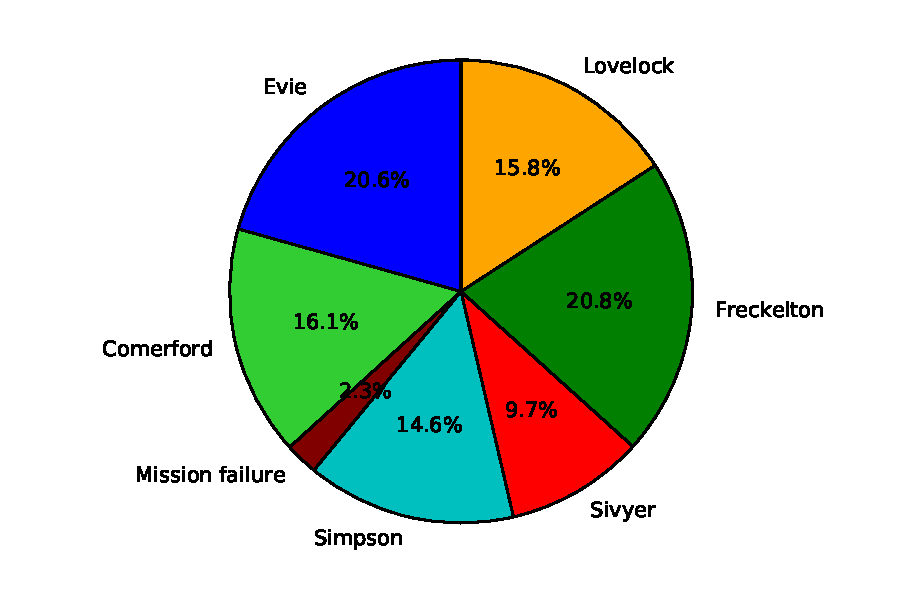
\includegraphics[width=\textwidth]{macro_analysis3.pdf}
		\caption{Fraction of asteroids mined per player.}
	\end{subfigure}
	\begin{subfigure}[b]{0.49\textwidth}
		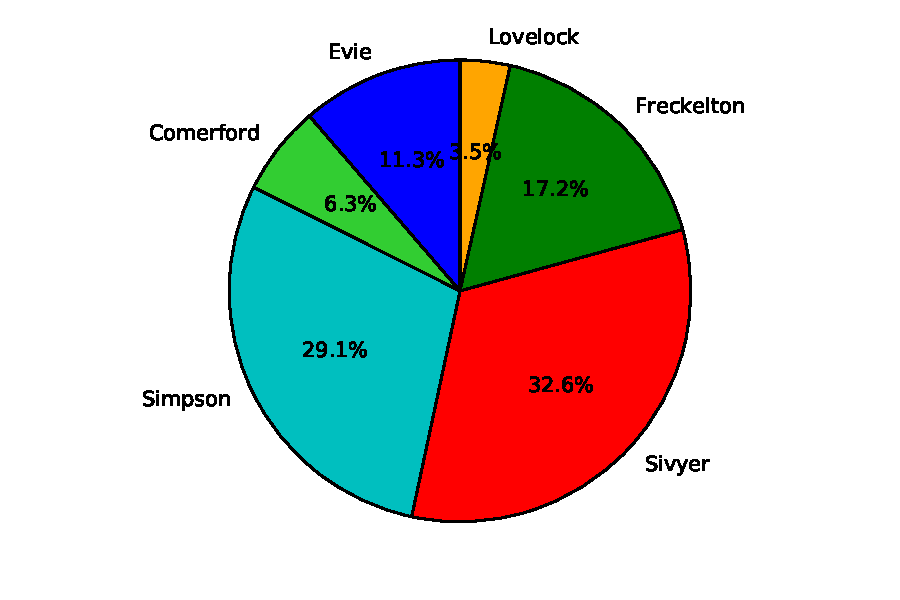
\includegraphics[width=\textwidth]{macro_analysis4.pdf}
		\caption{Final bankroll fraction per player.}
	\end{subfigure}
	\begin{subfigure}[b]{0.7\textwidth}
		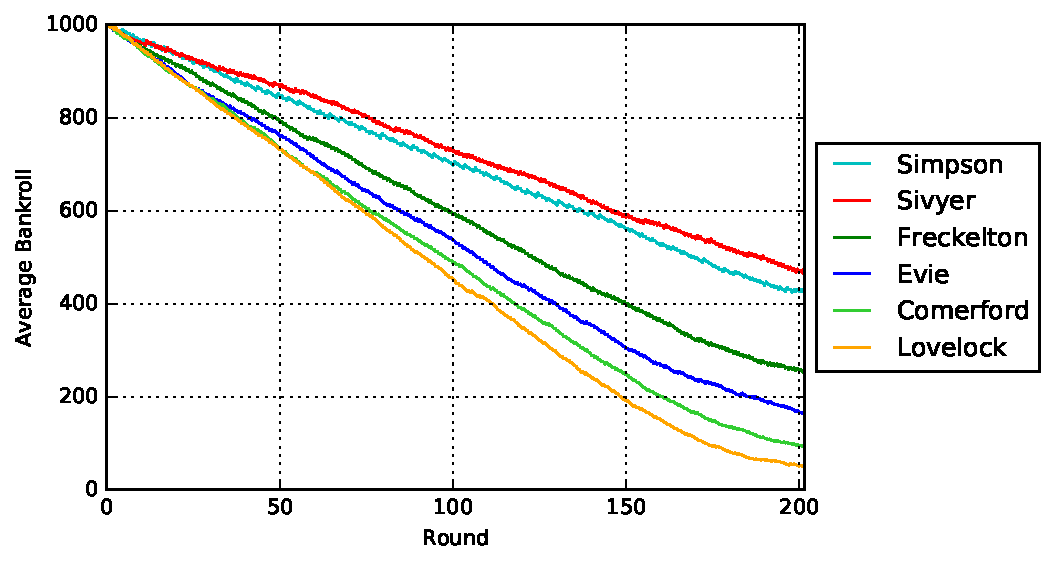
\includegraphics[width=\textwidth,keepaspectratio]{macro_analysis1.pdf}
		\caption{Average bankroll per round per player.}
	\end{subfigure}
	\caption{Analysis of the final form strategy taken from a random sample of 100 games.}
	\label{Analysis2}
\end{figure}

\subsection{The Cooperation Experiment}
A primary goal of player modelling is to avoid launching with other players, and thus maximize the chance at winning asteroids. An experiment was conducted between players Sivyer, Lovelock, and Simpson, to find out if a cooperative strategy could be successful. All three players agreed to consistently bid one in auctions and launch every third turn (for the nuances of this strategy, see Appendix B). The potential strength of this cooperative strategy was that members never competed with each other. As well as this, each player built up tech for three turns before launching, giving high mining probabilities.

Figure \ref{Analysis3} shows an averaged analysis for the three players running this code across 250 games. It can be seen that all players conducting the experiment have very similar scores, which is to be expected. Any difference is likely caused by starting on different rounds being beneficial or detrimental. By working together with very simple strategies, the group as a whole can be seen to get a large share of the final bankroll (71.5\%). This is a very high score and it shows that a group can control a large amount of the profit in \textit{Asteroid Mining Poker}. Comparing the cooperation strategy to the individual strategy uploaded (shown in Figure \ref{Analysis2}), it can be seen that cooperation with other players is worse for the individual. This can be observed by looking at the final bankroll scores. For player Sivyer, both the absolute final bankroll value, and the final bankroll fraction, were lower when playing in the group. This shows that, although working in a group can promote success, playing an individual strategy can grant even higher returns. This is a great example of the prisoner's dilemma: if there is no incentive to maximize a groups profits, the individual should act at the expense of the group \cite{axelrod1980effective}.

\begin{figure}[t]
	\centering
	\begin{subfigure}[b]{0.42\textwidth}
		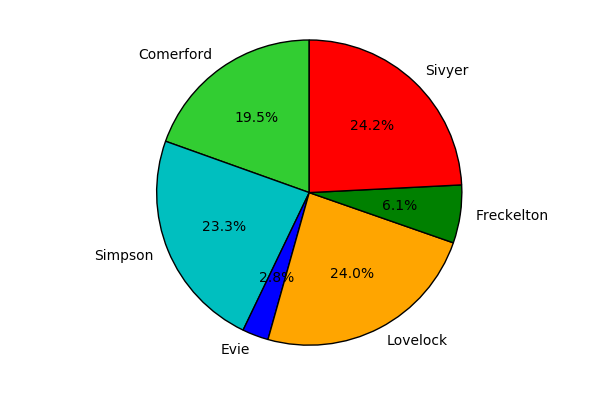
\includegraphics[width=\textwidth]{cartel_analysis4.png}
		\caption{Final bankroll fraction per player.}
	\end{subfigure}
	\begin{subfigure}[b]{0.57\textwidth}
		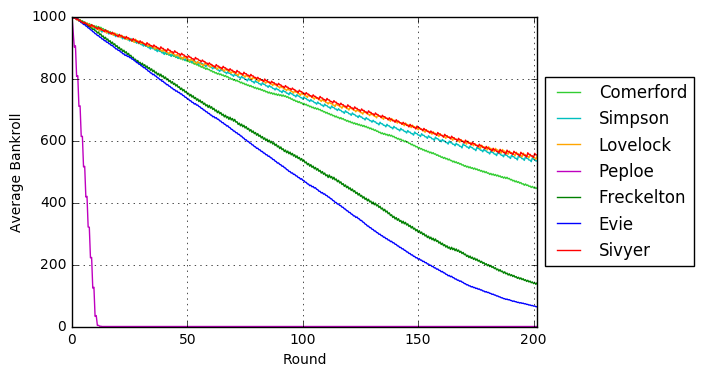
\includegraphics[width=\textwidth,keepaspectratio]{cartel_analysis1.png}
		\caption{Average bankroll per round per player.}
	\end{subfigure}
	\caption{Analysis of the cooperation strategy taken from a random sample of 250 games.}
	\label{Analysis3}
\end{figure}

To highlight the major flaw of using a cooperative strategy for a non-cooperative game, a new strategy was developed to mimic the cooperation strategy. This strategy played the same as the cooperation, but with a few changes. This strategy did not launch for asteroid with a value below four, and it always launched for asteroids with a value above 20. As well as this, the strategy launched for all asteroids early when just the cooperation members were left in the game (for the nuances of this strategy, see Appendix B). Figure \ref{CartelBoss} shows one game where this strategy was used while other players continued to use the cooperation strategy.

Analysis of figure \ref{CartelBoss} shows the effectiveness of a strategy that exploits other predictable strategies. This affirms conclusions made so far, as well as affirming the importance of a reliable player model: if the actions of other players is known (or can be predicted), they can be exploited for a large profit.

\begin{figure}[h!]
	\centering
	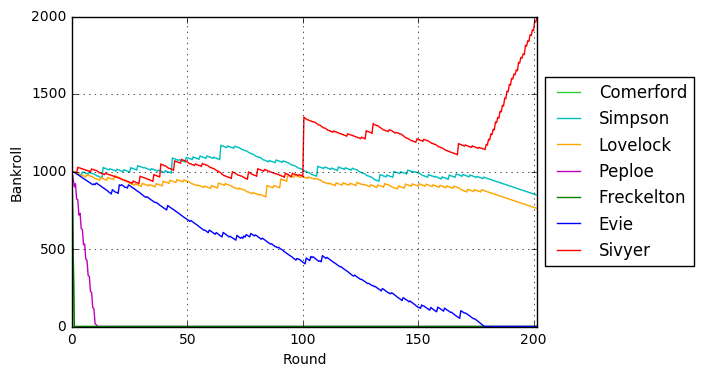
\includegraphics[width=0.8\textwidth,keepaspectratio]{cartel_boss.png}
	\caption{Bankroll per player per round. This game was run using the \textit{cooperation boss} strategy.}
	\label{CartelBoss}
\end{figure}

\newpage

\section{Findings} \label{Section4}

Total scores were calculated by totalling player's final bankrolls for the games at the end of each day. Because of this, the key result can be displayed by tracking these bankrolls. Figure \ref{GameHistory} shows the cumulative bankroll scores along with key events across the development of the final strategy. A function for this can be seen in \textit{the program} (see Appendix A).

\begin{figure}[h]
	\centering
	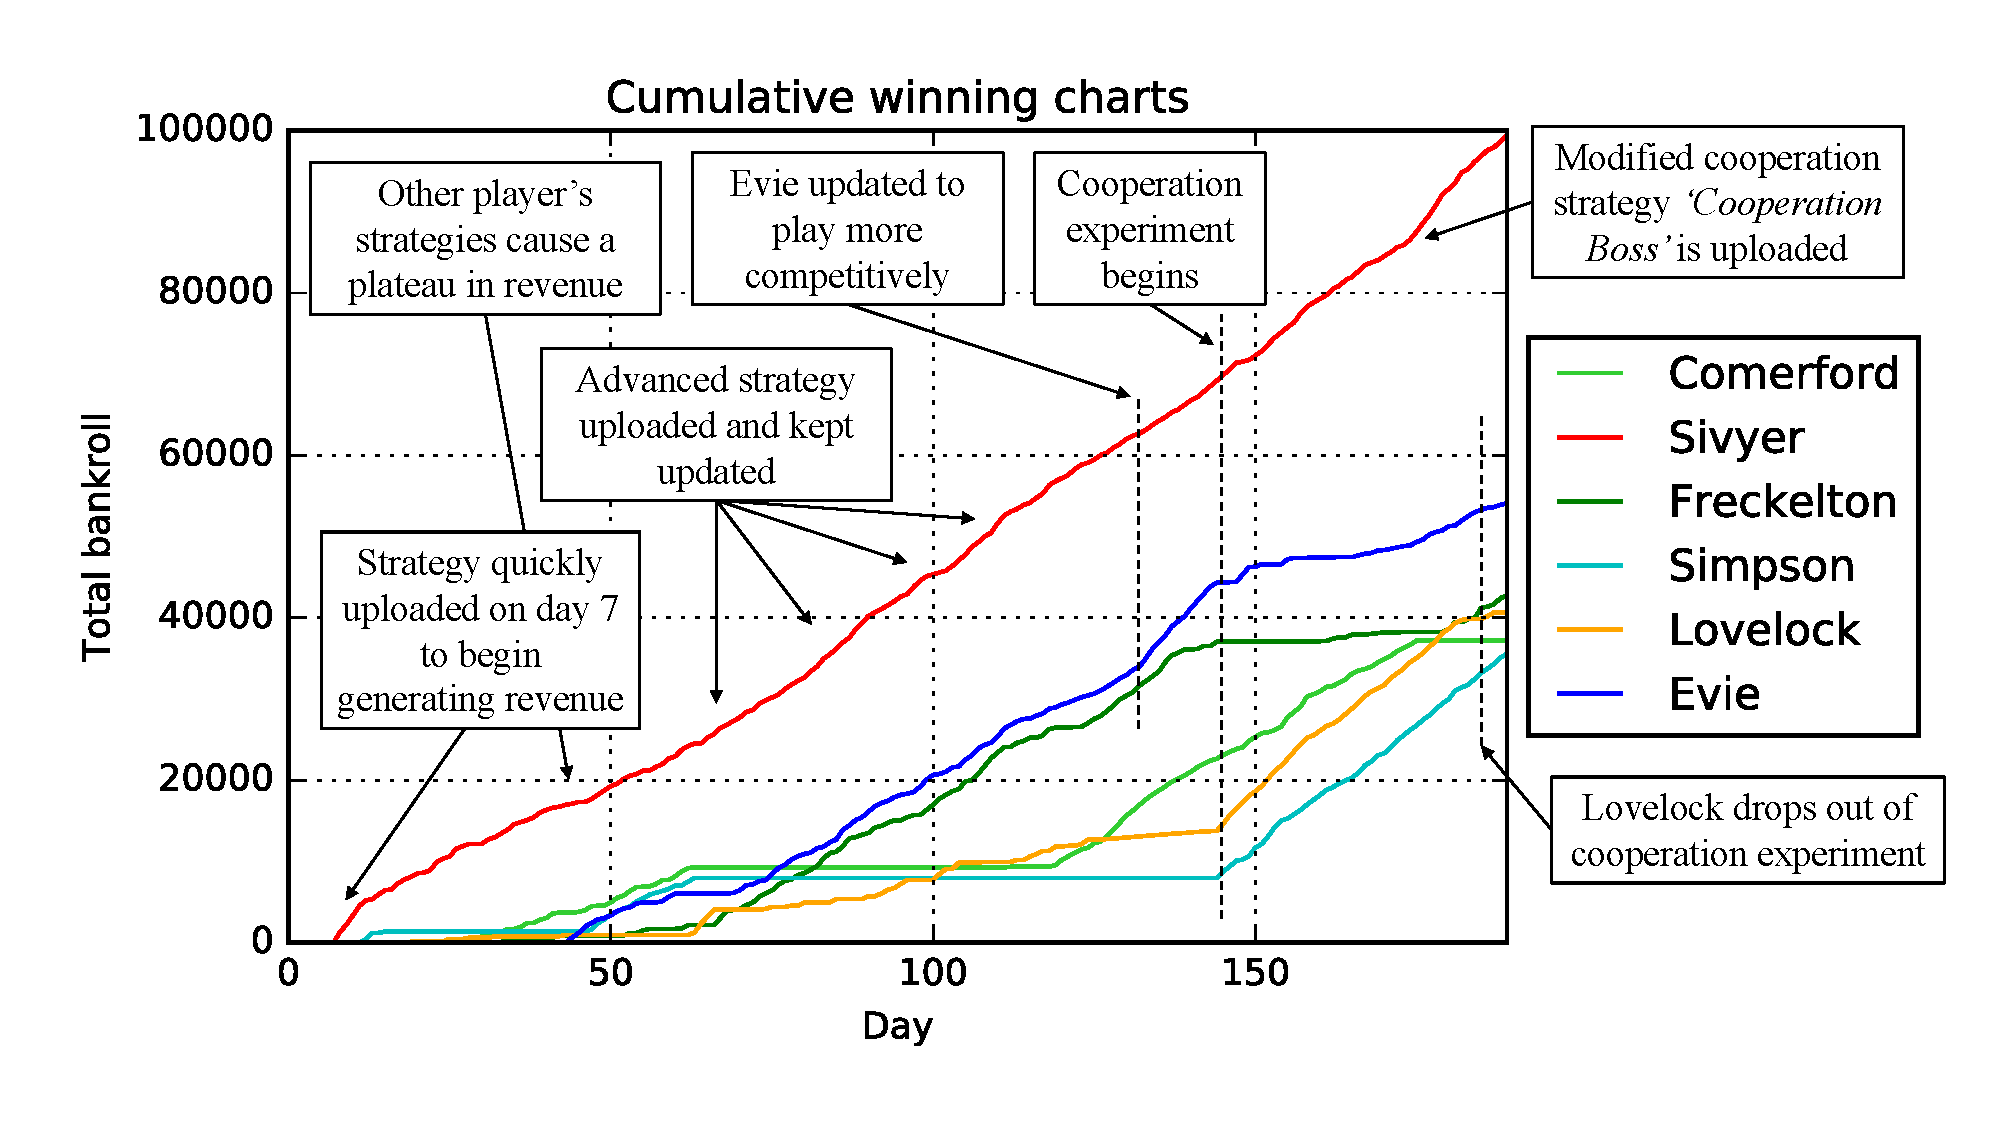
\includegraphics[width=\textwidth, keepaspectratio]{HistoryOfReport.pdf}
	\caption{Cumulative bankroll scores recorded from the 10$^{\text{th}}$ October through to the 18$^{\text{th}}$ April. Key events are highlighted. To see an enlarged variant, see Appendix D.}
	\label{GameHistory}
\end{figure}

As seen in Figure \ref{GameHistory}, by continually updating strategies a constant lead was maintained throughout the project. This shows that the principles applied in Section \ref{Section22} were good metrics to achieve success in the model. These principles combined logic, game theory, mathematical analysis, and machine learning techniques. These metrics were pitted against other players employing different strategies including cooperation, simple patterns, and their own game theoretical analysis. This shows that a successful strategy in \textit{Asteroid Mining Poker} has to employ multiple techniques and be adaptive to change in order to succeed. 

One particular aspect of Figure \ref{GameHistory} makes one thing very clear: the importance of consistency. There were many strategies that at one point or another, had a greater gradient than the strategy developed in this report (for example, Lovelock's strategy on day 70). Despite this, these strategies were not consistent and had large periods of inactivity. This meant that although other strategies may have been temporally successful, they failed to fully capitalize on that success. This is very similar to real world markets: economic success can be thwarted by bad management. This shows that consistency is a key factor for success in \textit{Asteroid Mining Poker}.

The four strategies shown in Figure \ref{GameHistory} will now be briefly reviewed, accompanied by an explanation of why they succeeded. Starting with the simple strategy, this strategy was effective because by usually bidding four, a cooperative standard was set up for the auctions \cite{lebrun1996existence}. When the strategy bid five, it modelled a simple prisoner's dilemma (by bidding five it was essentially 'defecting’, gaining the upper hand for the round it launched). This strategy only worked for a time however: when the competition became more advanced it stopped being effective, as it modelled predictable behaviour.

The advanced strategy used a heuristic player model to predict others' moves, a key component to winning non-cooperative games \cite{nash1951non}. On top of this, it was adaptive to new strategies played; being able to adjust the player model for any new behaviour observed. Finally, the strategy used data collected from the game itself to calculate the best possible chance it had to maximize bankroll fraction. By combining these techniques, this strategy was continuously successful. This increases confidence that bankroll fraction was the right standard at which to measure success. Also, this shows applying real world game theory is effective to do well in the game, verifying the effectiveness of the game as a model for economic activities.

The cooperation strategy attained a consistent bankroll. However, it had the issue that other players benefited equally. Because the aim was to find a strategy that maximizes the bankroll (which is valued against other players), playing a cooperative strategy was not successful. This showed that cooperation is a good technique for a group, but not for the individual in this model.

The findings from the cooperation strategy can be backed up by the final strategy experimented with: the cooperation boss strategy. This strategy had the highest gradient of bankroll for all the strategies developed as part of this project. This is because it made a profit at the expense of other players playing the cooperation strategy. However, this had the same problem as the cooperation strategies: it still had reliance on players using the cooperation strategy (as can be seen by Lovelock's change in strategy at the end of Figure \ref{GameHistory} which lead to a drop in bankroll gradient). This shows that exploiting other players may be the best way to gain bankroll quickly in the model, however this is very risky and requires other players to upload complementary strategies.

\subsection{Final Jersey Scores}

The jerseys were awarded based on the metrics shown in Table \ref{tab:jersey}. Final jersey scores as of 15$^{\text{th}}$ June 2019 can be seen in Table \ref{tab:JerseyFinals}. Study of Table \ref{tab:JerseyFinals} shows that all jersey awards were successfully attained by implementation of the strategies developed. This is beyond expectations and fulfils the strategy objective set out in Section \ref{sec:aims}.

\begin{table}[t!]
	\centering
	\caption{Final jersey scores for each player.}
	\label{tab:JerseyFinals}
	\begin{tabular}{lcccc}
		\toprule
		\textbf{Player} & \textbf{Yellow Jersey} & \textbf{Polka Dot Jersey} & \textbf{White Jersey} & \textbf{Green Jersey}\\
		\midrule
		Sivyer & 77 & 3 & 170 & 93012\\
		Evie & 25 & 1 & 123 & 53890\\
		Lovelock & 19 & 0 & 92 & 39070\\
		Simpson & 18 & 1 & 71 & 34400\\
		Comerford & 17 & 0 & 87 & 37194\\
		Freckelton & 16 & 1 & 94 & 41381\\
		Peploe & 2 & 0 & 14 & 2987\\
		\bottomrule
	\end{tabular}
\end{table}

Although the strategy objective only applied to the green jersey, applying game theory to successive strategies won all of the jersey awards. This may be because a strategy that can consistently accumulate the highest bankroll will also win the game most of the time, giving it the yellow and polka dot jerseys. Consistency is the key here, a risky strategy that gained an average higher bankroll with a higher variance, may only have won just the green jersey. This shows that a strategy optimizing for bankroll fraction will also be a consistent strategy. This may also explain why white jersey was attained as well (won for having the least bankruptcies).

\subsection{Suggested Improvements to the Strategy}
The final strategy could have been improved by removing various assumptions. For example, in multiple places the assumption that only one player wins the auction was made. This could be improved by using the average number of players who win auctions. Alternatively, the strategy could record the average number of auction winners for various asteroid base values, and make a prediction based off the data.

\subsection{Limitations of the Model}
Throughout development of strategies, a few limitations became clear. One major limitation is mentioned in Section \ref{Section22}: the game does not allow complex calculations due to a time out mechanism. In real world applications, a significant amount of time is allocated to making big economic decisions. A normal space mission takes years of planning (typically 2 -- 3 years \cite{davis2015long}). Hence, by having a short time out, the model cannot accurately represent calculations made in the industry. Because of this limitation, a full MCTS could not be applied to the advanced strategy which would have negatively affected its performance as a simplified calculation had to be used.

Another limitation of the model was the inability to upload multiple strategies at the same time. This is because it would have been useful to collect data by pitching strategies against each other. For example, the cooperation strategy could have been tested to see how its performance changed with group size.

\subsection{Applying the Model to Asteroid Mining} \label{sec:FindingsAM}
This section is consolidates data acquired and discusses how well \textit{Asteroid Mining Poker} can be applied to asteroid mining. This is done by comparing scientific results against the experimental observations made in Section \ref{sec:analysis1}.

\textit{Asteroid Mining Poker} models near-Earth asteroid (NEA) mining. This is because each asteroid can be mined in a given window of opportunity, similar to NEA's (and unlike asteroids from the asteroid belt) \cite{sonter2006asteroid}. The game models opportune times to mine these asteroids simply by having one appear continuously. This does not reflect the actual near-Earth environment where the distribution of NEA's is largely unknown, however it has been modelled \cite{bottke2000understanding}. Despite this, the game does not use any models to determine the frequency of asteroid appearance. The game also does not model the different locations and orbital positions of NEA's, reducing the applicability of the game.

Space missions have many variables and often fail. Mission failure is modelled in \textit{Asteroid Mining Poker} as a probability that decreases over time. Considering just one player launching every turn, who purchases no tech, the success chance is equal to $\frac{5}{F}$. Using the values of F discovered in Section \ref{sec:analysis1}, this would give a starting success rate (round one) of 60.4\% and an ending success rate (round 201) of 95\%. A case study can be made by considering similarly pioneering endeavours: the space missions to Mars. As of May 2019, there have been 58 missions to Mars \cite{MarsExpl75:online}. For the first ten of these, eight failed, giving a success rate of just 20\%. Of the last ten of these, only three have failed, giving a success rate of 70\%. The game successfully models an increase in success rate, however, the initial and final success rates may be too high as they do not reflect space mission history. 

The game models asteroid values by using two log normal distributions. As more data is made available on the value of asteroids, it would be ideal to confirm the value of NEA's does fall into a log normal distribution. However, due to a lack of significant data (since asteroids have not yet been mined), this cannot be confirmed. Despite this, the make up of an asteroid may appear known, but without significant tools and analysis, it's true value cannot be determined until it is mined. This is what the hidden distribution models, which is and increases applicability of the model.

In the analysis of successful strategies, it was noted that strategies almost always lost money. Many reports on asteroid mining conclude that there does not currently exist the technology to make asteroid mining profitable \cite{ross2001near}. This is modelled well by the game, which makes profit a very difficult goal.

\newpage

\section{Conclusion}

Through the development of a strategy and an analysis program, \textit{Asteroid Mining Poker} was successfully experimented with to: provide solid data on how the game worked, to show what strategies won success in it, and to determine how well the game represented asteroid mining.

The main aim of the project was accomplished: a strategy was developed that successfully applied game theoretical approaches to consistently win the green jersey award. These were set to measure what techniques were successful in the model. These techniques are discussed in Section \ref{Section4}, and include: consistency, adaptability, application of theory, and the application of data. One of the primary factors in a good strategy was found to be an accurate player model, as would be expected for non-cooperative games.

The secondary aim was also fulfilled. By discovering all unknown distributions in the game, the model was then compared with asteroid mining in an engineering context. It was shown that the model is very simplified and does not include many of the engineering challenges that face the industry. This has the benifit of being easy to run and experiment with, as complex models would require significantly more computer power.

All objectives were met. A strategy was developed which incorporated game theoretical approaches. It then went on to successfully and consistently win the green jersey award through the application of a player model. On top of this, an analysis program showed how the game worked by determining all the unknowns. It also analysed outputted logs in order to visualize and improve the strategy. Finally, it was able to analyse multiple logs and find averages in place of a short-term jersey system. The fulfilment of these objectives further shows the aims were achieved.

\subsection*{Future Areas of Research}
Future research could focus on applying engineering challenges to the game. These could include:

\begin{itemize}
	\item Limited number of bidding rounds to simulate companies missing the opportunity window to mine a passing near Earth asteroid.
	\item No asteroid appearance for some rounds to model times when there are no asteroid launch opportunities.
	\item Launch cost variation for asteroids modelled in different orbital planes.
\end{itemize}

As well as this, the game could be made more complex to see if this would effect the techniques required by a successful strategy. Such changes could include:

\begin{itemize}
	\item Random number of rounds to prevent strategies always launching on the last round.
	\item More information about who is launching to make the \textit{join launch} option viable.
	\item Allow testing with multiple strategies per player.
	\item Increase calculation time allowed to experiment with more complex strategies.
\end{itemize}

Any number of these implementations may improve the model and make it a more viable tool to experiment with the economics of asteroid mining. The development of these models is very important for potential industries without experimental data. Finding out what strategies succeed in certain environments can give a huge advantage to the one employing them and enable a head start in the industry.

% BIBLIOGRAPHY
\newpage
\bibliographystyle{ieeetr}
\bibliography{References}

%APPENDIX
\newpage
\section{Appendices}
\renewcommand{\thesubsection}{\thesection.\alph{subsection}}
\subsection*{A. The Python Program}
\addcontentsline{toc}{subsection}{A.\hspace{0.6cm} The Python Program}

The program is structured as a series of functions that can be called via a console. All functions begin with detailed instructions on how to use them. The full code is available for download at \url{https://github.com/CodingWithJack/AsteroidMiningPoker}.

Table \ref{tab:pstructure} displays all the functions in the program along with what they do (table excludes functions intended only to be used by the program itself).

\begin{longtable}{p{0.2\textwidth}p{0.6\textwidth}}
	\caption{Functions included in the program and what they do.}\\
	% first head
	\toprule \textbf{Function name} & \textbf{Basic operation} \\ \midrule
	\endfirsthead
	% second head & continued
	\multicolumn{1}{l}{\textit{Table continued from last page.}}\\
	\toprule \textbf{Function name} & \textbf{Basic operation} \\ \midrule \endhead
	% first foot onwards
	\bottomrule \multicolumn{1}{l}{\textit{Table continued on next page.}} \endfoot
	% last foot
	\bottomrule \endlastfoot
	% Content
	get\_local\_log & Downloads latest local log. \\
	get\_global\_log & Downloads the latest global log. \\
	get\_daily\_logs & Downloads all logs recorded at the end of the day up to (but not including) the date called. \\
	auto\_log & Downloads the latest local log every 10 minutes. \\
	get\_file & Downloads any named file from the client server. \\
	upload\_strategy & Uploads a file to the online server as 'strategies.py'. \\
	create\_clean\_json & Creates or replaces a json file named 'compiled\_data.json' (needed to pool data for analysis functions) \\
	compile\_data & Compiles and saves important data from a local log into 'compiled\_data.json'. The log is then moved to a new location specified. \\
	base\_dist & Plots a graph showing the probability function for the base value of the asteroids. \\
	hidden\_dist & Plots a graph showing the probability function for the hidden value of the asteroids. \\
	base\_tech & Plots a graph showing the probability distribution of the tech gained at the start of each round. \\
	auction\_tech & Plots a graph showing the probability distribution of tech gained after winning an auction. \\
	tech\_function & Plots a graph showing the change of the average total reward of asteroids against the tech launched by all players. \\
	round\_failure & Plots a blue bar chart showing the total observed distribution of tech spent by all players against frequency for a single round. Red bars are also plotted representing rounds observed which ended in a \textit{Mission failure} win. \\
	failure\_tech & Plots a graph showing the estimated \textit{Mission failure} probability for 201 rounds. \\
	daily\_wins & Plots a graph showing the final bankrolls all games recorded at the end of each day. Plot the bankroll variation for the past 10 days by default. \\
	plot\_bankroll & Plots the variation of bankroll for the beginning of each round across any game. \\
	analyse & Plots various graphs associated with a log. In order of appearance these are: tech variation per round for all players, bankroll per round for all players, base value and auction price of asteroids per round, percent of auctions won per player, money spent of auctions per player, fraction of tech committed per player, fraction of asteroids mined per player, and fraction of final bankroll per player. \\
	macro\_analysis & Plots various graphs associated with the past n logs. In order of	appearance these are: average bankroll per round for all players, average fraction of tech committed per player, average fraction of asteroids mined per player, and average fraction of final bankroll per player.
	\label{tab:pstructure}
\end{longtable}

\subsection*{B. Strategies}
\addcontentsline{toc}{subsection}{B.\hspace{0.6cm} Strategies}

Throughout the project, four strategies were developed. This appendix is concerned with detailing these strategies. A strategy can only return three things: a bid amount, a decision to launch, and a decision to join a launch (as seen in Figure \ref{GameVisual}). The logic for each of these decisions is detailed for simple strategies. All strategies are available for download at \url{https://github.com/CodingWithJack/AsteroidMiningPoker}.

\subsubsection*{Basic Strategy}
Operation dates: 17$^{\text{th}}$ October 2018 to 10$^{\text{th}}$  December 2018.

Strategy overview: This strategy was good at mining asteroids quickly when there was little competition. However, it quickly became ineffective as other players uploaded competitive strategies (see Figure \ref{GameHistory}).

Launch decision: The launch decision was set to True if the tech was greater than 4 and the base value greater than 5 or if the tech value was greater than 10. It was set to false in all other cases.

Bid amount: The bid amount was set to five if the launch decision was True. Otherwise, it was set to four.

Join launch decision: This was always set to False.

\subsubsection*{Final Strategy}
Operation dates: 10$^{\text{th}}$ December 2018 to 27$^{\text{th}}$ March 2019.

Strategy overview: This strategy was very successful at maximizing the bankroll gained ahead of other players. Using game theoretical approaches with logical deductions, this strategy was able to achieve all possible awards.

Launch decision and bid amount: Reviewed in Section \ref{SectionDEVSTRAT}.

Join launch decision: This was always set to False.

\subsubsection*{Cooperation Strategy}
Operation dates: 27$^{\text{th}}$ March 2019 to 8$^{\text{th}}$ April 2019.

Strategy overview: This strategy successfully modelled cooperation with other players to achieve a consistently good score. This strategy had the issue of being reliant on other players having to upload the same strategy, making it vulnerable to being exploited. 

Launch decision: The launch decision was based on the remaining number of members in the cooperation. Each member took turns to launch starting with the first player alphabetically.

Bid amount: The bid amount was set to one if there were remaining members outside the cooperation. Otherwise, the bid amount was set to zero.

Join launch decision: This was always set to False.

\subsubsection*{Cooperation Boss Strategy}
Operation dates: 8$^{\text{th}}$ April 2019 to 1$^{\text{st}}$ May 2019 (project end).

Strategy overview: This strategy successfully showed the failure of cooperative strategies in non-cooperative games. This was done by modelling the cooperation strategy, with a few alterations. By applying situational analysis to maximize it's own bankroll, this strategy achieved a consistently good score at the expense of the other players running the cooperation strategy.

Launch decision: In most circumstances, this followed the launch pattern of the cooperation strategy. However, if the asteroid base value fell below four, the strategy did not launch. Also, if the asteroid base value rose above 20, the strategy always chose to launch.

Bid amount: In general, the bidding behaviour was the same as the regular cooperation strategy. However, if an asteroid with a base value above 20 appeared, the strategy would bid two.

Join launch decision: This was always set to False.


\subsection*{C. Data Visualizations}
\addcontentsline{toc}{subsection}{C.\hspace{0.6cm} Data Visualizations}

For any game, a variety of data visualizations were developed. These were based on the metrics perceived to give the most useful information about the game. This appendix shows what data visualizations were made, why they were made, and gives an example of their use.

\begin{longtable}{p{0.3\textwidth}p{0.3\textwidth}p{0.3\textwidth}}
	\caption{Analysis tools developed and why they were produced.}\\
	% first head
	\toprule \textbf{Data visualisation} & \textbf{Reason for visual} & \textbf{Example of use} \\ \midrule
	\endfirsthead
	% second head & continued
	\multicolumn{1}{l}{\textit{Table continued from last page.}}\\
	\toprule \textbf{Function name} & \textbf{Basic operation} \\ \midrule \endhead
	% first foot onwards
	\bottomrule \multicolumn{1}{l}{\textit{Table continued on next page.}} \endfoot
	% last foot
	\bottomrule \endlastfoot
	% Content
	Line graph showing tech variation per round (for all players). & Can see a player's tech spending habits. & Regular patterns and maximum tech values become obvious. \\
	Line graph showing bank variation per round. & Can see trends in bankroll. & Can see the effect that one player going bankrupt has on the other players. \\
	Line graph showing per round variation of base reward, final auction price, and normalised tech price. & Can see average auction price in a game along with the change in auction price for different base values. & Can judge a good auction price by that spent by other players who do not go bankrupt. \\
	Horizontal bar chart showing percentage of auctions won in a game per player. & Can see which players are bidding in the auctions and how often. & Can see if a players investments are paying off by comparing to final bankroll pie chart. \\
	Horizontal bar chart showing bankroll committed to auctions in a game per player .& Can see how much bankroll players are committing to additional tech. & Can compare to percentage of auctions won horizontal bar chart to see which players are getting the most tech for the lowest price. \\
	Pie chart showing fraction of tech committed in a game per player. & Can see how much tech each player has accumulated and committed throughout a game. & Can compare to final bankroll pie chart to see which players are using their tech at the right time. \\
	Pie chart showing fraction of asteroids mined in a game per player. & Can see how many asteroids each player is mining per game. & Can tell if players are going for cheap asteroids often, or expensive asteroids rarely, or a bit of both \\
	Pie chart showing fraction of final bankroll in a game per player. & Can see how successful each player's strategy is. & Can compare to other statistics to get an idea as to the source of the winner's success. \\
	\label{tab:analysis}
\end{longtable}

\subsection*{D. Key Result Enlarged}
\addcontentsline{toc}{subsection}{D.\hspace{0.6cm} Key Result Enlarged}

Figure \ref{GameHistoryENLARGED} shows an enlarged version of Figure \ref{GameHistory}, to allow for deeper analysis and discussion.

\begin{figure}[h]
	\centering
	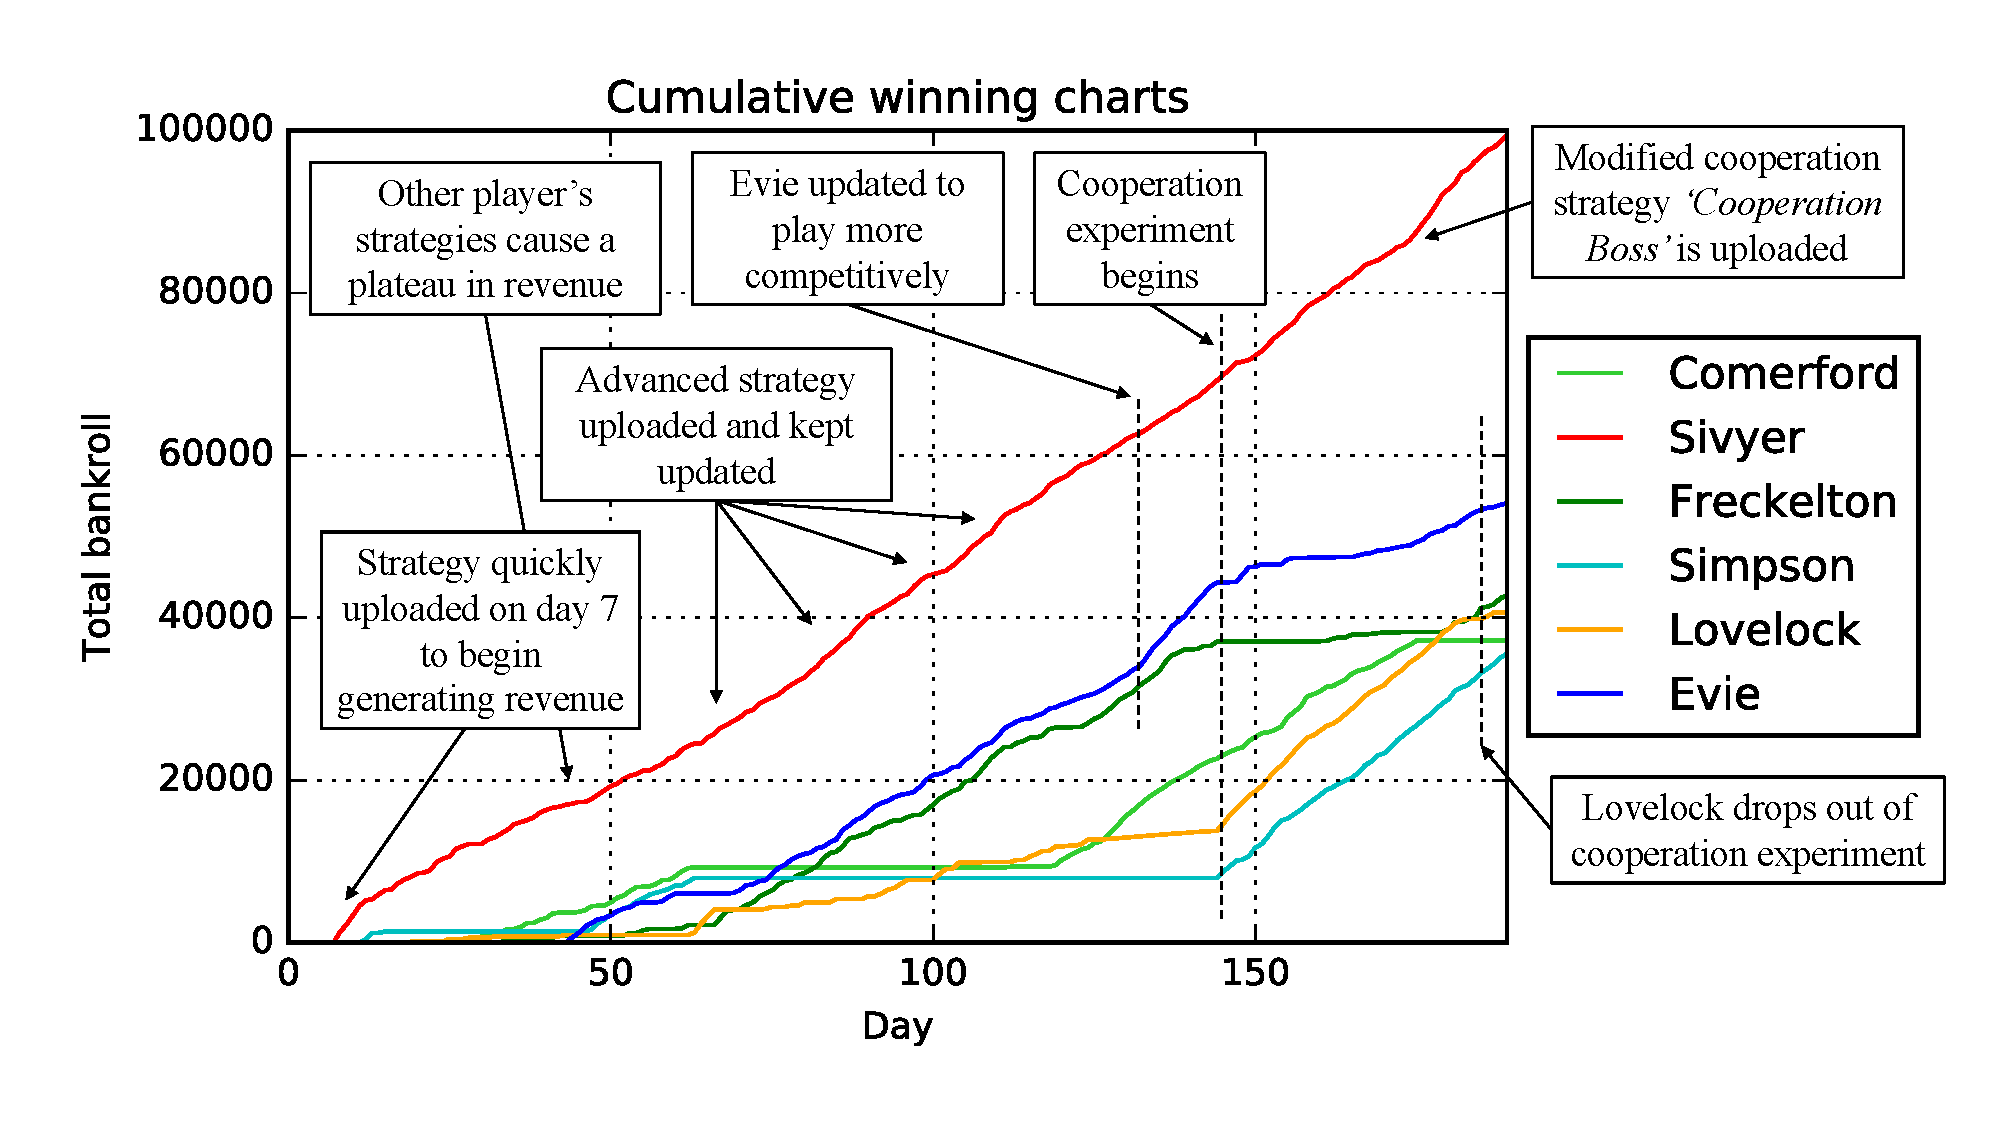
\includegraphics[width=0.9\textheight, keepaspectratio, angle=90]{HistoryOfReport.pdf}
	\caption{Cumulative bankroll scores recorded from the 10$^{\text{th}}$ October through to the 18$^{\text{th}}$ April. Key events are highlighted. Enlarged variant for Figure \ref{GameHistory}.}
	\label{GameHistoryENLARGED}
\end{figure}

\end{document}
